\documentclass[11pt]{article}

\usepackage[margin=1in]{geometry}
\usepackage{graphicx}
\usepackage{multirow}
\usepackage{amsmath,amssymb,amsfonts}
\usepackage{amsthm}
\usepackage{xcolor}
\usepackage{textcomp}
\usepackage{booktabs}
\usepackage{tabularx}
\usepackage[version=4]{mhchem}
\usepackage{epstopdf}
\usepackage[mathlines]{lineno}
\usepackage{setspace}
\usepackage{etoolbox}
\usepackage[colorlinks=true,allcolors=blue]{hyperref}
\hypersetup{pdftitle={Electrochemical Design Basis for Titanium Production by Mg--Ca Co-Deposition in a Quaternary Chloride Melt}, pdfauthor={Yaming Hu}}

\graphicspath{{figures_eps/}}

\AtBeginEnvironment{table}{\singlespacing}

\begin{document}

\linenumbers
\doublespacing

\title{Electrochemical Design Basis for Titanium Production by Mg--Ca Co-Deposition in a Quaternary Chloride Melt}

\author{Yaming Hu\thanks{Independent Researcher, Guiyang, Guizhou Province, China. E-mail: 64687555@qq.com}}

\date{}

\maketitle

\begin{abstract}
This work establishes an electrochemical design basis for titanium production by in situ co-deposition of Mg and Ca, cyclic reductants of $\ce{TiO2}$, in a quaternary chloride melt ($\ce{MgCl2}$--$\ce{CaCl2}$--NaCl--KCl). Thermodynamics at 600~$^{\circ}$C gives $\Delta G^{\circ} = -231.0$ to $-307.5$~kJ/mol for the reduction pathways, with deoxidation limits of 3908~ppm O for Mg and 20.2~ppm for Ca ($\approx$77~ppm at the equimolar alloy activity). $\ce{Ca + MgO -> CaO + Mg}$ is exergonic at 600~$^{\circ}$C ($\Delta G^{\circ} = -38.2$~kJ/mol; $K = 194$), so Ca supplies the deoxidation driving force while Mg keeps the reductant liquid (both pure metals are solid at 600~$^{\circ}$C; the Mg--Ca eutectic melts at $\approx$517~$^{\circ}$C), reaching the deep-deoxidation limit only when $a_{\ce{MgO}} < 5\times10^{-3}$. The $\ce{Ca^{2+}/Na+}$ co-deposition window is 120.2~mV (ideal) and remains positive under activity-coefficient sensitivity, and mass transport limits Mg deposition to 0.56~A/cm$^2$: co-deposition spans 0.56--1.31~A/cm$^2$, the equimolar deposit requires $j \approx 1.1$~A/cm$^2$, and the 0.9~V ohmic budget constrains the gap to $\lesssim$1.1~cm. The shrinking-core model predicts complete reduction of 100~$\mu$m particles in 6.3~min. At the nominal design point ($\eta_I = 0.75$, $V_{\mathrm{cell}} = 4.1$~V) the net equivalent energy is 12{,}552~kWh/ton-Ti, or 12{,}933~kWh/ton-Ti ($+$3\%) if CaO rather than MgO--CaO is regenerated---the mechanistically favoured limit, since $\ce{Ca + MgO -> CaO + Mg}$ generates no solid product layer, with the 1:1 balance retained as the conservative basis; both are \emph{conditional on achieving $\eta_I > 0.70$}. Monte Carlo gives medians of 13{,}141 and 13{,}536~kWh/ton-Ti ($P(W<15{,}000) = 82.1\%$ and 76.6\%, which mainly restates the assumed $\eta_I$ prior). All results are theoretical; viability hinges on adequate $\ce{CaO}$ solubility at 600~$^{\circ}$C, on whether MgO is regenerated electrolytically or reduced chemically by Ca, on melt oxoacidity favouring $\ce{O2}$ over $\ce{Cl2}$, and on a durable inert anode.
\end{abstract}

\vspace{0.2em}
{\small\noindent\textbf{Keywords:} titanium production; molten salt electrolysis; Mg--Ca co-deposition; deoxidation; process design\par}

\newpage

\section*{Introduction}

Titanium is a strategic material for aerospace, marine engineering, and energy applications owing to its low density, high specific strength, and exceptional corrosion resistance. However, widespread civilian use remains limited by high production costs. The Kroll process, the dominant industrial route, requires multiple batch operations---chlorination, magnesiothermic reduction, and vacuum distillation---resulting in high energy consumption, severe pollution, and intermittent production \cite{kroll1937,ji2026}.

The core challenge in titanium metallurgy lies in the extremely high Ti--O bond energy, making efficient deoxidation difficult, while titanium's chemical reactivity at elevated temperatures leads to contamination by N, H, and C. Molten salt electrolysis has emerged as a promising alternative. The FFC (Fray--Farthing--Chen) Cambridge process \cite{fray2000} directly reduces $\ce{TiO2}$ cathodically in $\ce{CaCl2}$ melt, but suffers from low current efficiency and difficult product separation. The USTB (University of Science and Technology Beijing) process \cite{jiao2023} uses electrochemical dissolution-deposition of titanium anodes but faces anode durability issues. The OS process \cite{ono2002} performs calciothermic reduction of $\ce{TiO2}$ in $\ce{CaCl2}$ melt with electrolytic regeneration of Ca, sharing the ``electrolytic regeneration of reductant'' concept with the present work. The SOM process \cite{pal2001} employs a solid oxide membrane to separate the anode from the melt, achieving higher current efficiency. Okabe et al.\ \cite{okabe1997} developed the electronically mediated reaction (EMR) approach for titanium production. Several review articles have summarized recent progress \cite{ji2026,zhang2024}.

Recent studies have explored $\ce{MgCl2}$-based salt systems for titanium production. Taninouchi et al. \cite{taninouchi2016} demonstrated electrochemical deoxidation of titanium in molten $\ce{MgCl2}$. Lim et al. \cite{lee2025} investigated $\ce{CaMg2}$ as a reductant for $\ce{TiO2}$. Pang et al. \cite{pang2024} achieved ultralow-oxygen titanium by direct reduction. Zhu et al. \cite{xu2025} produced low-oxygen titanium powder by molten salt electrolysis--magnesiothermic reduction. However, these approaches employ either single-metal reductants or preformed (off-line synthesized) bimetallic reductants such as $\ce{CaMg2}$, operate in binary/ternary salt systems, and rely on batch operation with preformed cathodes, differing in salt composition, reduction mechanism, and operational design from the in-situ co-deposition process proposed here.

This paper proposes a quaternary $\ce{MgCl2-CaCl2-NaCl-KCl}$ molten salt system enabling in-situ electrolytic co-deposition of Mg and Ca for complementary reduction of $\ce{TiO2}$. The key innovation is an electrochemical-thermochemical coupling: the co-deposited Mg--Ca alloy serves as a cyclic liquid reductant, in which the alloy provides a liquid reductant phase at 600~$^{\circ}$C---both pure metals are solid at that temperature---while Ca supplies the thermodynamic driving force for deep deoxidation, CaO being the stable oxide. The by-product oxides ($\ce{MgO}$, $\ce{CaO}$) dissolve in the $\ce{CaCl2}$-containing melt and are electrolytically regenerated, establishing a closed-loop cycle. This work presents a systematic thermodynamic, electrochemical, and kinetic assessment using established databases \cite{barin1995,waldner1999} and literature parameters, providing a quantitative theoretical framework. The specific novelties of this study are:

\begin{itemize}
\item To the authors' knowledge, the first proposal of in-situ electrolytic co-deposition of Mg and Ca in a quaternary $\ce{MgCl2-CaCl2-NaCl-KCl}$ molten salt for titanium production, combining a liquid Mg--Ca reductant phase---which is what allows operation at 600~$^{\circ}$C, where both pure metals are solid---with Ca's thermodynamic deoxidation depth in a single closed-loop process. While bimetallic Mg--Ca reductants (e.g., $\ce{CaMg2}$ \cite{lee2025}), $\ce{MgCl2}$-based deoxidation \cite{taninouchi2016}, and electrolytic Ca regeneration in the OS process \cite{ono2002} have been studied, the in-situ electrolytic co-deposition of both Mg and Ca in a quaternary system is novel at the process-integration level: the individual unit operations---alloy co-deposition, metallothermic reduction, oxide dissolution, and electrolytic regeneration---are each established, but their in-situ coupling within a single quaternary melt is not.
\item Alloy mixing behavior is characterized using the CALPHAD-derived Redlich--Kister parameters of the Mg--Ca system from the assessment of Zhang et al.\ \cite{zhang2008mgce}, rather than an ideal-solution assumption. Additionally, the robustness of the $\ce{Ca^{2+}/Na+}$ co-deposition window is evaluated by combining Nernst-equation calculation, activity-coefficient sensitivity analysis, and overpotential qualitative analysis, and a cathode diffusion-layer analysis (limiting current densities, Mg--Ca co-deposition regimes, and the ohmic-drop cell-geometry constraint) converts the equilibrium window into an operating current-density design map.
\item Kinetic prediction via the shrinking core model with multi-parameter sensitivity analysis ($D = 1$--$3\times10^{-9}$~m$^2$/s, $\varepsilon = 0.1$--0.5, $\tau = 1.5$--5.0), providing reduction time estimates for process design.
\item Full-process energy balance analysis (12{,}552~kWh/ton-Ti net equivalent consumption at the nominal design point, or 12{,}933~kWh/ton-Ti if Ca is the sole net oxygen carrier, the case favoured by the mechanism analysis; \emph{both theoretical predictions conditional on achieving $\eta_I > 0.70$}; process energy efficiency 48.7\%, second-law efficiency 36.3\%, electrolysis energy fraction 97.2\%) with preliminary comparison to both Kroll and FFC routes, acknowledging boundary differences.
\end{itemize}

This work is a conceptual feasibility study conducted independently: all thermodynamic, electrochemical, and kinetic calculations, data processing, and uncertainty analyses were performed computationally by the author from published data and open-source tooling, without access to institutional laboratory facilities. The results are therefore intended as a quantitative design basis for subsequent experimental validation.

\newpage

\section*{Nomenclature}

\begin{singlespace}
\small
\begin{tabular}{ll}
\multicolumn{2}{l}{\textit{Thermodynamic quantities}} \\
$\Delta G^{\circ}$ & Standard Gibbs free energy change (kJ/mol) \\
$\Delta H^{\circ}$ & Standard enthalpy change (kJ/mol) \\
$\Delta S^{\circ}$ & Standard entropy change (J/(mol$\cdot$K)) \\
$\Delta G_{\mathrm{mix}}$ & Mixing Gibbs free energy of Mg--Ca alloy (kJ/mol) \\
$\Delta G_{\mathrm{deox}}$ & Deoxidation free energy, per 1~mol O basis (kJ/mol) \\
$\Delta G_{\mathrm{diss}}$ & Dissolution free energy of O in $\alpha$-Ti (J/mol) \\
$\Delta H_{\mathrm{fus}}$ & Enthalpy of fusion (kJ/mol) \\
$C_p$ & Heat capacity (J/(mol$\cdot$K)) \\
$K$ & Equilibrium constant \\
\multicolumn{2}{l}{\textit{Electrochemical quantities}} \\
$E^{\circ}_{\mathrm{red}}$ & Standard reduction potential (V) \\
$E_{\mathrm{red}}$ & Reduction potential (V) \\
$E_d$ & Decomposition voltage (V) \\
$\Delta E$ & Co-deposition window (mV) \\
$n$ & Number of electrons transferred \\
$a$ & Activity \\
$\gamma$ & Activity coefficient \\
$p_{\ce{O2}}$ & Oxygen partial pressure (atm) \\
\multicolumn{2}{l}{\textit{Physical constants}} \\
$R$ & Universal gas constant, 8.314 J/(mol$\cdot$K); particle radius in SCM section (m) \\
$F$ & Faraday constant, 96{,}485 C/mol \\
\multicolumn{2}{l}{\textit{Process variables}} \\
$T$ & Temperature (K or $^{\circ}$C as indicated) \\
$T_m$ & Melting temperature (K) \\
$x_i$ & Mole fraction of component $i$ \\
$j$ & Current density (A/cm$^2$) \\
$j_{\mathrm{lim}}$ & Limiting current density (A/cm$^2$) \\
$j_0$ & Exchange current density (A/cm$^2$) \\
$\delta$ & Cathodic diffusion-layer thickness ($\mu$m) \\
$\kappa$ & Melt electrical conductivity (S/cm) \\
$L$ & Interelectrode gap (cm) \\
$D$ & Diffusion coefficient (m$^2$/s) \\
$D_{\mathrm{eff}}$ & Effective diffusion coefficient, $D\varepsilon/\tau$ (m$^2$/s) \\
$\varepsilon$ & Porosity \\
$\tau$ & Tortuosity \\
$c_{\mathrm{O}}$ & Oxygen concentration in TiO$_2$ (mol/m$^3$) \\
$c_{\mathrm{red}}$ & Reductant concentration (mol/m$^3$) \\
$M_{\mathrm{avg}}$ & Effective molar mass of the reductant-bearing melt ($\approx$93 g/mol) \\
$\eta_I$ & Current efficiency \\
$V_{\mathrm{cell}}$ & Cell voltage (V) \\
$\Omega$ & Interaction parameter (kJ/mol) \\
$L_0$ & Zeroth-order Redlich--Kister parameter (J/mol; text quotes kJ/mol at 873~K) \\
$L_1$ & First-order Redlich--Kister parameter (J/mol, neglected in this work) \\
$w_{[\mathrm{O}]}$ & Equilibrium oxygen content (wt\%) \\
$p_{\mathrm{O}^{2-}}$ & Negative logarithm of oxide ion activity, $-\log_{10}(a_{\mathrm{O}^{2-}})$ \\
$n_{\mathrm{Ti}}$ & Moles of Ti per metric ton ($\mathrm{mol/ton}$) \\
\end{tabular}
\end{singlespace}

\newpage

\section*{Process Description}

The proposed process is designed over a 580--650~$^{\circ}$C operating range, with 600~$^{\circ}$C taken as the nominal \emph{design-basis} temperature at which all thermodynamic and kinetic figures herein are reported. Because of the liquidus uncertainty (Limitations~(4)), a pilot-scale operating floor of $\geq$620~$^{\circ}$C is recommended; the shift from 600 to 620~$^{\circ}$C changes the energy and co-deposition-window figures by only a few percent and does not alter the qualitative conclusions. The melt is a quaternary $\ce{MgCl2-CaCl2-NaCl-KCl}$ mixture. $\ce{MgCl2}$ serves as the primary salt and magnesium source; $\ce{CaCl2}$ enhances oxide solubility and lowers the melting point; NaCl and KCl act as fluxes to improve ionic conductivity and reduce viscosity \cite{sato1999}. The recommended composition ($x_{\ce{MgCl2}} = 0.30$, $x_{\ce{CaCl2}} = 0.40$, $x_{\ce{NaCl}} = x_{\ce{KCl}} = 0.15$) is derived in the Salt Composition Design section from three requirements: a liquidus at least 30~$^{\circ}$C below the operating floor, a $\ce{Ca^{2+}/Na+}$ co-deposition window above 50~mV, and sufficient $\ce{CaCl2}$ to dissolve the by-product oxides. The operational cycle consists of: (i) electrolytic co-deposition of Mg and Ca at the cathode; (ii) reduction of $\ce{TiO2}$ powder by the co-deposited metals, with Ca supplying the thermodynamic driving force and Mg keeping the reductant liquid (Eq.~\ref{eq:camgo}); (iii) dissolution of the by-product oxides in the melt; and (iv) electrolytic regeneration of the reductant with oxygen evolution at the anode---MgO and CaO in Case~II of Table~\ref{tab:mbalance}, predominantly CaO if Ca acts as the sole net oxygen carrier. In a continuously operated cell these four processes proceed concurrently in the same vessel; the numbering expresses the functional charge and material flow, not a temporal sequence. Electrolysis and the $\ce{TiO2}$ feed are continuous, but the solids are not: because both the Ti product and the unreacted oxide settle, the cell is operated semi-continuously, the settled bed being drained periodically through a bottom isolation valve while fresh $\ce{TiO2}$ is fed to its surface (see the Reactor Configuration section). The net reaction is $\ce{TiO2 -> Ti + O2}$, driven by electrical energy, with Mg and Ca acting as cyclic mediators.

\begin{figure}[!ht]
\centering
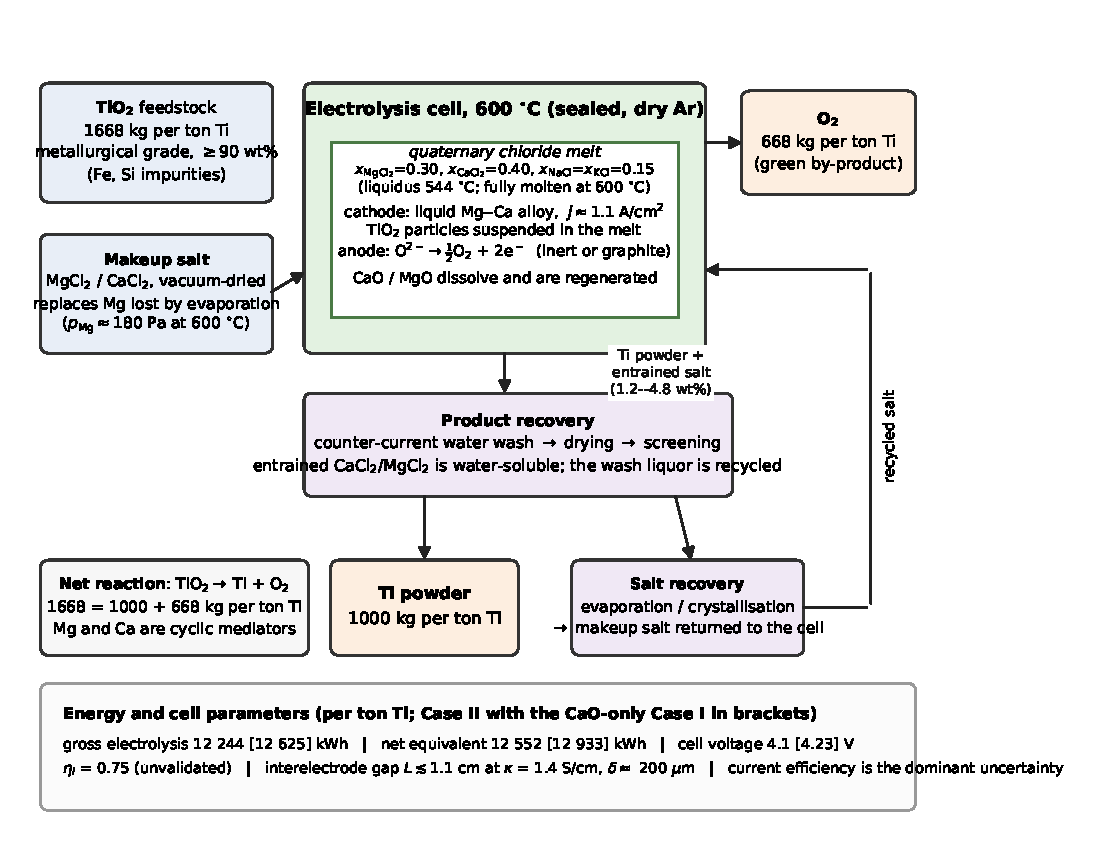
\includegraphics[width=0.86\linewidth]{figure_flowsheet.eps}
\caption{Process flowsheet of the proposed route. Case~II material and energy figures are given, with the CaO-only Case~I values in brackets. Metallurgical-grade $\ce{TiO2}$ powder settles onto the cathode floor of the quaternary chloride melt; the cathode co-deposits the liquid Mg--Ca reductant within the settled bed, which reduces the particles in situ; the by-product oxides dissolve and are electrolytically regenerated at the anode with oxygen evolution; the Ti powder is recovered by water washing and the salt is recycled.}
\label{fig:flowsheet}
\end{figure}

\subsection*{Feedstock, Reactor Concept and Product Recovery}

\textbf{Feedstock.} All figures use pure $\ce{TiO2}$ as the balance basis; the metallurgical-grade case ($\geq$90~wt\% $\ce{TiO2}$, $\sim$186~kg of Fe/Si impurities per ton Ti) is treated in the E--$p\ce{O^{2-}}$ section, with the deliberately excluded impurity-separation energy quantified in Limitations~(7).

\textbf{Reactor concept.} The cell is a single sealed vessel at 600~$^{\circ}$C under dry argon. Because liquid Ti is 2.5 times denser than the melt---a 100~$\mu$m particle settles at $\approx$5~mm/s (Stokes, $Re \approx 0.3$), traversing a 20~cm melt in under a minute---the product cannot be held in suspension by mild circulation, and circulation vigorous enough to suspend it would carry conductive Ti powder into the anode region. The cell is therefore configured so that reaction, current collection and product accumulation share one location: the crucible floor, or a conductive liner embedded in it, serves as the current collector; the settled $\ce{TiO2}$ forms a conductive bed that extends the cathode into the particle assembly; and the reductant is electrodeposited within that bed, where capillarity retains it against buoyancy (the Mg--Ca alloy, $\approx$1.6~g/cm$^3$, is lighter than the 1.8~g/cm$^3$ melt and would otherwise float). The inert anode is suspended in the clear melt above and enclosed in a porous ceramic shroud that keeps the bed, or solids entrained by anodic gas evolution, out of the interelectrode gap. At production scale the geometry cannot remain a crucible with a central anode---the ohmic budget below would demand an anode almost as wide as the cell, leaving no lateral path for anodic gas and no access for drainage---so the production configuration is a horizontal plate anode suspended $\sim$1~cm above the bed, with gas escaping past the plate edges and the crucible acting as container and current collector rather than as the principal cathode surface. Cathode and anode must be closely spaced: the 0.9~V ohmic budget is met only for $L \lesssim 1.1$~cm at $j \approx 1.1$~A/cm$^2$ and $\kappa = 1.4$~S/cm (Fig.~\ref{fig:current_regimes}b), making a close-spaced or diaphragm-integrated assembly a requirement rather than an option. The anode must evolve $\ce{O2}$ rather than $\ce{Cl2}$ (Fig.~\ref{fig:cl2}) while resisting $\ce{O^{2-}}$ and $\ce{Cl^-}$ attack (Limitations~(8)). Because Mg has an appreciable vapour pressure at 600~$^{\circ}$C ($\approx$180~Pa), the freeboard must be sealed and the Mg vapour condensed and returned, which also keeps the alloy's Mg inventory in steady state (Cathode Mass Transport section).

\textbf{Product recovery.} The product is a porous Ti powder that inherits the external dimensions of the 25--100~$\mu$m precursor and settles on the cell floor rather than forming a coherent cathode deposit, so recovery is a solid--liquid separation followed by a dry solid--solid separation. A 1~$\mu$m salt film on 25--100~$\mu$m powder corresponds to $\approx$11~wt\% (25~$\mu$m) down to $\approx$3~wt\% (100~$\mu$m) of entrained salt; as $\ce{CaCl2}$ and $\ce{MgCl2}$ are highly water-soluble, counter-current washing and drying remove the salt at of order 0.5--1.5~m$^3$ of wash water per ton Ti. The washed powder is nonetheless a mixture of metallic Ti and unreacted $\ce{TiO2}$ of essentially the same particle size, so screening alone cannot separate them; it is retained only to recycle the coarsest, least-reacted particles. Separation relies on the conductivity contrast---metallic Ti is an electronic conductor and $\ce{TiO2}$ an insulator---and is performed by dry electrostatic separation, preceded by gentle ultrasonic or gas-jet liberation of the friable Ti shell (milling is excluded: it would oxidise the product and destroy the size contrast on which classification depends). Where metallurgical-grade feedstock is used, reduced Fe and Si report partly as the free metals and are removed by high-gradient magnetic separation and mild alkaline leaching respectively, although intermetallic formation with Ti (Limitations~(7)) limits the efficiency of both steps. The separated oxide fraction is returned to the cell as feedstock, and all dry steps are enclosed under argon. The wash liquor is evaporated and the salt returned to the cell, so the ``post-treatment'' line of the energy balance is a pumping and drying duty (Limitations~(7) distinguishes it from impurity removal).

\subsection*{Reactor Configuration and Semi-Continuous Operation}

Three constraints fix the cell architecture: the density contrast that makes the product settle, the need to keep the reductant in contact with the particles, and the requirement that conductive solids never bridge the interelectrode gap. They are met at a single location, as set out under Reactor concept: a sloped floor acting as current collector, a settled bed that extends the cathode into the particle assembly, and a shroud-isolated anode in the clear melt above.

Gravity drainage is preferred to mechanical extraction for three reasons: a 620~$^{\circ}$C slurry of abrasive oxide and metal powder rapidly destroys pump internals; pumping disturbs the bed and can lift conductive Ti powder towards the anode; and a dynamic seal at the cell floor is the most probable leak path in a sealed chloride cell. The floor is therefore sloped to a single port and the slurry is drained in batches, which is why the process is described as semi-continuous rather than continuous. The slope itself is a design target rather than a measured quantity (Limitations~(11)).

The interelectrode gap is fixed by the ohmic budget at $L \lesssim 1.1$~cm, which rules out an otherwise obvious expedient---separating the anode from the bed by a large distance. At $j = 1.1$~A/cm$^2$ and $\kappa = 1.4$~S/cm a 10~cm gap would dissipate 7.9~V, tripling the cell voltage and erasing the energy advantage over the Kroll route (Fig.~\ref{fig:current_regimes}b). Short-circuit protection must therefore be geometric rather than dimensional: the shroud excludes the bed from the gap, and the bed height is controlled by drainage frequency rather than by a fixed freeboard.

Operation follows a fixed sequence. The salts are vacuum-dehydrated and melted; electrolysis is started in the absence of solids to establish the reductant inventory; and particulate $\ce{TiO2}$ is admitted only once a liquid reductant phase exists, since admitting an insulating oxide beforehand gives no reduction and risks blocking the current path. Thereafter feed and electrolysis are continuous while the bed is drained periodically.

\textbf{Melt state at the design temperature.} All four pure salts melt above 600~$^{\circ}$C ($\ce{MgCl2}$ 714, $\ce{CaCl2}$ 772, KCl 770, NaCl 801~$^{\circ}$C), so the design temperature appears to lie below the melting range of every constituent. In a quaternary mixture, however, the liquidus is depressed by the entropy of mixing: applying the liquidus condition of Eq.~\ref{eq:liquidus} component by component gives 543.7~$^{\circ}$C, controlled by $\ce{CaCl2}$---the value quoted in the Salt Composition Design section---so the melt is fully liquid at 600~$^{\circ}$C with 56~$^{\circ}$C of superheat. The open question is therefore not whether the melt is liquid, but by how much the ideal-solution liquidus underestimates the real one (Limitations~(4)).

\section*{Process Comparison}

Table~\ref{tab:compare} compares the proposed process with established technologies. The key distinction is the electrochemical-thermochemical coupling: unlike FFC (pure electro-deoxidation) or Kroll (pure metallothermic), this process uses electrolysis to regenerate the reductant in situ while leveraging a liquid Mg--Ca alloy in which Ca supplies the thermodynamic deoxidation depth and Mg keeps the reductant molten at 600~$^{\circ}$C, where both pure metals are solid. The 600~$^{\circ}$C operating temperature is 300--350~$^{\circ}$C below the FFC route ($\sim$950~$^{\circ}$C) and the OS process ($\sim$900~$^{\circ}$C); that reduction is what the liquid alloy buys, and it lowers thermal losses and material corrosion without changing the thermodynamically required decomposition voltage.

\begin{table}[!ht]
  \centering
  \caption{Comparison of titanium production processes}
  \label{tab:compare}
  \footnotesize
  \setlength{\tabcolsep}{3pt}
  \begin{tabularx}{\linewidth}{@{} p{1.5cm} p{2.5cm} p{1.4cm} p{1.2cm} p{1.4cm} p{1.3cm} X @{}}
  \toprule
  Process & Core Principle & Mode & Temp. ($^{\circ}$C) & Energy & Purity & Key Challenge \\
  \midrule
  Kroll & Chlorination + Mg reduction & Batch & 1000--1200 & Very high & High & Long process, pollution \\
  FFC & Direct electro-deoxidation & Batch & $\sim$950 & High & Moderate & Low current efficiency \\
  OS & Electrolytic Ca regeneration + calciothermic reduction & Cyclic & $\sim$900 & High & High & Ca reactivity, high temp. \\
  SOM & Solid oxide membrane electrolysis & Semi-cont. & 700--800 & Moderate & High & Membrane durability \\
  USTB & Anode dissolution-deposition & Semi-cont. & $\sim$900 & High & High & Anode loss \\
  Proposed & In-situ Mg--Ca co-deposition; liquid Mg--Ca reductant with Ca as thermodynamic deoxidizer & Semi-cont. (conceptual) & 580--650$^{b}$ & Moderate$^{a}$ & High (target) & Anode corrosion, unvalidated $\eta_I$, Ca--MgO kinetics \\
  \bottomrule
  \end{tabularx}
  \par\vspace{2pt}
  \footnotesize $^{a}$Theoretical prediction conditional on $\eta_I > 0.70$. 12{,}552~kWh/ton-Ti assumes a MgO--CaO regeneration mixture; 12{,}933~kWh/ton-Ti assumes CaO as the sole regenerated species (Eq.~\ref{eq:camgo}). Industrial/pilot values shown for Kroll/FFC/USTB are not directly equivalent.
  $^{b}$Hard pilot operating floor of $\geq$620~$^{\circ}$C recommended (Limitations~(4)); 600~$^{\circ}$C is the design-basis temperature at which the reported figures are calculated.
\end{table}

\section*{Thermodynamic Framework}

\subsection*{Data Sources and Computational Methods}
\label{subsec:data}

All thermodynamic calculations use standard thermochemical data from Barin \cite{barin1995} and Kubaschewski and Alcock \cite{kubaschewski1979}, together with the CALPHAD (Calculation of Phase Diagrams) assessment of the Ti--O system by Waldner and Eriksson \cite{waldner1999}. Temperature-dependent Gibbs free energies are computed via the Gibbs-Helmholtz relation:
\begin{equation}
\label{eq:gibbs}
\Delta G^{\circ}(T) = \Delta H^{\circ}(T) - T\,\Delta S^{\circ}(T)
\end{equation}
where $\Delta H^{\circ}(T)$ and $\Delta S^{\circ}(T)$ are obtained by integrating $C_p$ from 298~K (Kirchhoff law: $d\Delta H/dT = \Delta C_p$), accounting for phase transitions (Mg: $T_m=923$~K, $\Delta H_{\mathrm{fus}}=8.95$~kJ/mol; Ca: $T_m=1115$~K, $\Delta H_{\mathrm{fus}}=8.54$~kJ/mol). The Nernst equation is used for electrochemical analysis:
\begin{equation}
\label{eq:nernst}
E_{\mathrm{red}} = E^{\circ}_{\mathrm{red}} + \frac{RT}{nF}\ln(a_{\mathrm{M}^{n+}})
\end{equation}
The standard-state data from Barin \cite{barin1995} are compiled for the range 298--1000~K; their use at 873~K (600~$^{\circ}$C) involves Cp extrapolation through the solid--liquid transition for Mg and Ca, which is expected to introduce an uncertainty of approximately $\pm$1--2~kJ/mol in $\Delta G^{\circ}$. All calculations are implemented in Python with CSV output for data traceability.

\subsection*{Salt Composition Design and Liquidus Estimation}

The liquidus temperature of the quaternary system is estimated using the ideal solution model. For each component $i$, the liquidus condition is:
\begin{equation}
\label{eq:liquidus}
x_i \le \exp\!\left[-\frac{\Delta H_{\mathrm{fus},i}}{R}\left(\frac{1}{T} - \frac{1}{T_{m,i}}\right)\right]
\end{equation}
with $T_{m,i}$ and $\Delta H_{\mathrm{fus},i}$ for $\ce{MgCl2}$ (987~K, 43.1~kJ/mol), $\ce{CaCl2}$ (1045~K, 28.5~kJ/mol), NaCl (1074~K, 28.2~kJ/mol), and KCl (1043~K, 26.6~kJ/mol). The recommended composition ($x_{\ce{MgCl2}}=0.30$, $x_{\ce{CaCl2}}=0.40$, $x_{\ce{NaCl}}=0.15$, $x_{\ce{KCl}}=0.15$) yields a calculated liquidus of 544~$^{\circ}$C, 36~$^{\circ}$C below the target minimum operating temperature (Fig.~\ref{fig:liquidus}). The composition was selected based on three criteria: (i) the calculated liquidus must remain $>$30~$^{\circ}$C below the target operating temperature floor (580~$^{\circ}$C), providing a safety margin against freezing; (ii) the $\ce{Ca^{2+}/Na+}$ co-deposition window must exceed 50~mV (see the Activity Coefficient Sensitivity Analysis section); and (iii) the $\ce{CaCl2}$ content must be sufficient to dissolve the by-product oxides ($\ce{MgO}$, $\ce{CaO}$), based on the well-established solubility of alkaline earth oxides in $\ce{CaCl2}$-rich melts \cite{ono2002}. The selected composition satisfies all three: liquidus = 544~$^{\circ}$C (margin = 36~$^{\circ}$C), co-deposition window $\geq$74.9~mV across the full sensitivity range (Table~\ref{tab:window_sens}), and $x_{\ce{CaCl2}} = 0.40$ provides theoretically feasible oxide solubility pending 600~$^{\circ}$C experimental validation (see the Oxide Dissolution section).

\begin{figure}[!ht]
\centering
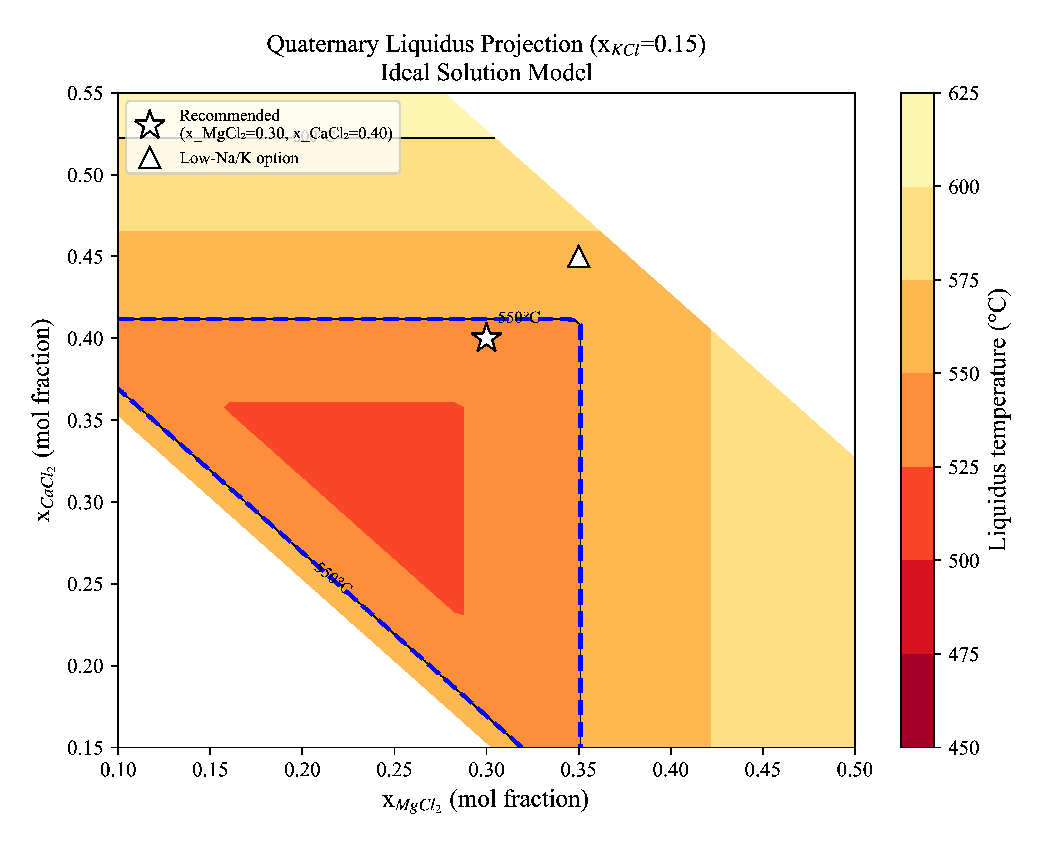
\includegraphics[width=0.95\linewidth]{figure1.eps}
\caption{Liquidus projection of the quaternary $\ce{MgCl2-CaCl2-NaCl}$ system at $x_{\ce{KCl}}=0.15$ (ideal solution model).}
\label{fig:liquidus}
\end{figure}

It should be noted that the ideal solution model does not account for solid miscibility gaps or intermediate compounds, and the actual liquidus may deviate substantially. Table~\ref{tab:binary} summarizes the six binary subsystems from the assessed phase diagrams of Chartrand and Pelton \cite{chartrand2000}: the $\ce{NaCl}$/$\ce{KCl}$-bearing binaries form low-melting compounds/eutectics (minimum liquidus $\sim$440--657~$^{\circ}$C) that \emph{depress} the liquidus, whereas the dominant $\ce{MgCl2-CaCl2}$ pair forms the congruently-melting compound $\ce{CaMg2Cl6}$ ($\approx$621~$^{\circ}$C) that \emph{raises} the liquidus above the ideal prediction. Because $\ce{MgCl2}$+$\ce{CaCl2}$ constitute 70~mol\% of the recommended composition, the net deviation is expected to be upward, consistent with the estimated $\pm$50~$^{\circ}$C uncertainty (upper bound $\sim$594~$^{\circ}$C). Precise prediction requires CALPHAD assessment with dedicated databases (e.g., FactSage SGTE or MTOX); the present calculation serves as a preliminary design guideline. The 36~$^{\circ}$C margin between the calculated liquidus (544~$^{\circ}$C) and the minimum operating temperature (580~$^{\circ}$C) may be insufficient if the actual liquidus exceeds 580~$^{\circ}$C, and a hard operating floor of $\geq$620~$^{\circ}$C (or CALPHAD confirmation of a lower liquidus) is recommended before pilot-scale implementation (see also Limitations~(4)).

\begin{table}[!ht]
\centering
\footnotesize
\caption{Co-deposition window sensitivity to activity coefficients at 600~$^{\circ}$C.}
\label{tab:window_sens}
\begin{tabular}{cccc}
\toprule
$\gamma_{\ce{CaCl2}}$ & $\gamma_{\ce{NaCl}}$ & Window (mV) & Assessment \\
\midrule
1.0 & 1.00 & 120.2 & Good \\
1.0 & 0.85 & 132.4 & Good \\
1.0 & 0.70 & 147.1 & Good \\
0.9 & 1.00 & 116.3 & Good \\
0.9 & 0.85 & 128.5 & Good \\
0.9 & 0.70 & 143.1 & Good \\
0.8 & 1.00 & 111.8 & Good \\
0.8 & 0.85 & 124.1 & Good \\
0.8 & 0.70 & 138.7 & Good \\
0.7 & 1.00 & 106.8 & Good \\
0.7 & 0.85 & 119.0 & Good \\
0.7 & 0.70 & 133.6 & Good \\
0.5 & 1.00 & 94.2 & Moderate \\
0.5 & 0.85 & 106.4 & Good \\
0.5 & 0.70 & 121.0 & Good \\
0.3 & 1.00 & 74.9 & Moderate \\
0.3 & 0.85 & 87.2 & Moderate \\
0.3 & 0.70 & 101.8 & Good \\
\bottomrule
\end{tabular}
\end{table}

\begin{table}[!ht]
\centering
\footnotesize
\caption{Binary subsystems of the quaternary salt and their minimum liquidus features (assessed phase diagrams \cite{chartrand2000}).}
\label{tab:binary}
\begin{tabular}{lcl}
\toprule
Binary system & Key phase(s) & Minimum liquidus ($^{\circ}$C) \\
\midrule
$\ce{MgCl2-NaCl}$ & $\ce{NaMgCl3}$, $\ce{Na2MgCl4}$ & $\sim$440 \\
$\ce{MgCl2-CaCl2}$ & $\ce{CaMg2Cl6}$ (congruent) & $\sim$621 \\
$\ce{CaCl2-NaCl}$ & simple eutectic & $\sim$500 \\
$\ce{CaCl2-KCl}$ & $\ce{KCaCl3}$ + eutectic & $\sim$600 \\
$\ce{MgCl2-KCl}$ & $\ce{KMgCl3}$, $\ce{K2MgCl4}$ & $\sim$470 \\
$\ce{NaCl-KCl}$ & solid solution & $\sim$657 \\
\bottomrule
\end{tabular}
\end{table}

\subsection*{Activity Coefficient Sensitivity Analysis}
\label{subsec:activity}

In the quaternary chloride melt, ion-ion interactions cause deviations from ideality ($\gamma \neq 1$). Experimental activity coefficient data for the quaternary $\ce{MgCl2-CaCl2-NaCl-KCl}$ system at 600~$^{\circ}$C are limited in the open literature. Thermodynamic optimization of the $\ce{MgCl2-NaCl}$ binary system \cite{chartrand2000} reports negative deviation ($\gamma < 1$) due to strong $\ce{Mg^{2+}-Cl^{-}}$ interactions. By analogy, $\ce{CaCl2-NaCl}$ and other charge-unsymmetrical chloride mixtures are expected to exhibit similar negative deviation, as established by Kleppa's thermochemical studies of charge-unsymmetrical halide melts \cite{kleppa1966}, though direct activity measurements in the quaternary system remain scarce. The modified quasichemical model (MQM) used in the FactSage Salt database \cite{pelton2000mqm} formally captures these effects, but the database parameters are not publicly available.

To assess the impact of non-ideality on the co-deposition window, a parametric sensitivity analysis is performed. The Nernst equation with activity correction becomes:
\begin{equation}
\label{eq:canernst}
E_{\mathrm{red}}(\ce{Ca^{2+}}) = E^{\circ}_{\mathrm{red}}(\ce{Ca^{2+}/Ca}) + \frac{RT}{2F}\ln(\gamma_{\ce{CaCl2}} \cdot x_{\ce{CaCl2}})
\end{equation}
\begin{equation}
\label{eq:naernst}
E_{\mathrm{red}}(\ce{Na+}) = E^{\circ}_{\mathrm{red}}(\ce{Na+/Na}) + \frac{RT}{F}\ln(\gamma_{\ce{NaCl}} \cdot x_{\ce{NaCl}})
\end{equation}

The co-deposition window $\Delta E = E_{\mathrm{red}}(\ce{Ca^{2+}}) - E_{\mathrm{red}}(\ce{Na+})$ is scanned over six $\gamma_{\ce{CaCl2}}$ values (1.0, 0.9, 0.8, 0.7, 0.5, 0.3) and three $\gamma_{\ce{NaCl}}$ values (1.0, 0.85, 0.7), covering the range from ideal behavior to strong negative deviation reported for charge-unsymmetrical chloride melts \cite{kleppa1966}. The results (Table~\ref{tab:window_sens}) show that the window remains positive (74.9--147.1~mV) across all 18 combinations, with 15 cases classified as ``Good'' ($>$100~mV) and 3 as ``Moderate'' (50--100~mV). Even at $\gamma_{\ce{CaCl2}} = 0.3$, the narrowest window (74.9~mV, with $\gamma_{\ce{NaCl}} = 1.0$) exceeds the 50~mV threshold for viable co-deposition. The critical $\gamma_{\ce{CaCl2}}$ at which the window vanishes is estimated at $\sim$0.02--0.04 (depending on $\gamma_{\ce{NaCl}}$), far below the smallest value ($\gamma_{\ce{CaCl2}} = 0.3$) employed in the sensitivity scan or reported for charge-unsymmetrical chloride mixtures \cite{chartrand2000,kleppa1966}. This is obtained by setting $\Delta E = 0$ in the Nernst equations (Eqs.~\ref{eq:canernst}--\ref{eq:naernst}), i.e., $E^{\circ}_{\mathrm{red}}(\ce{Ca^{2+}/Ca}) + (RT/2F)\ln(\gamma_{\ce{CaCl2}} \cdot x_{\ce{CaCl2}})$ $= E^{\circ}_{\mathrm{red}}(\ce{Na+/Na}) + (RT/F)\ln(\gamma_{\ce{NaCl}} \cdot x_{\ce{NaCl}})$, and solving for $\gamma_{\ce{CaCl2}}$ at $T = 873$~K with the recommended composition. The resulting $\gamma_{\ce{CaCl2}} \approx 0.02$--0.04 lies far below the scanned range, indicating that the recommended composition provides a robust co-deposition window even under significant non-ideality, pending CALPHAD validation or direct measurement.

Note that $\gamma_{\ce{CaCl2}}$ and $\gamma_{\ce{NaCl}}$ here denote component-scale activity coefficients of CaCl$_2$ and NaCl, obtained from binary-system measurements \cite{chartrand2000,kleppa1966}. In this work, component-scale activity coefficients are adopted for the Nernst-equation calculation as a feasible approximation, rather than ionic-scale activity coefficients. At high $\ce{CaCl2}$ fractions, the formation of $\ce{CaCl+}$ and $\ce{CaCl3-}$ associates breaks the full-dissociation assumption, which will cause deviation of ionic-scale activity from component-scale activity. This qualitative understanding of Ca--O association is consistent with the short-range-ordering framework adopted in the FactSalt MQM model developed by Pelton et al.\ \cite{pelton2000mqm}, in which ion-pair interactions are considered for molten-salt thermodynamic calculation. This approximation is only used for preliminary evaluation of the co-deposition window, and future MQM-based calculation can separate component activity and ionic activity precisely.

\subsection*{Mg--Ca Liquid Alloy Thermodynamic Parameters}
\label{subsec:MgCa}

The in-situ co-deposited Mg--Ca forms a liquid alloy at 600~$^{\circ}$C (above the Mg--Ca eutectic at $\approx$517~$^{\circ}$C). The Mg--Ca system has been assessed by Nayeb-Hashemi and Clark \cite{nayeb1987} and re-assessed by Zhang et al. \cite{zhang2008mgce} using the CALPHAD method. The liquid phase is described by a Redlich--Kister expansion:
\begin{equation}
\label{eq:rk}
G^{\mathrm{ex}}_{\mathrm{Mg-Ca}} = x_{\mathrm{Mg}}x_{\mathrm{Ca}}\left[L_0 + L_1(x_{\mathrm{Mg}}-x_{\mathrm{Ca}})\right]
\end{equation}
The formation of the stable intermetallic $\ce{Mg2Ca}$ indicates exothermic mixing. The Ca--Mg liquid Redlich--Kister parameters (standard SGTE database values, compiled in the collection of Hallstedt \cite{hallstedt2025}) are adopted here following the CALPHAD assessment of Zhang et al. \cite{zhang2008mgce}: $L_0 = -30616 + 13.72\,T$~J/mol and $L_1 = -532 + 2.70\,T$~J/mol. At 600~$^{\circ}$C (873~K), $L_0 = -18.64$~kJ/mol. Using a regular solution approximation ($L_1 = 0$, $\Omega \approx L_0$ with $\Omega$ frozen at its 873~K value), the mixing enthalpy at equimolar composition is $-4.66$~kJ/mol (the Kirchhoff-corrected value using the full $L_0(T)$ form is $-7.65$~kJ/mol), consistent with the assessed phase diagram and the $\ce{Mg2Ca}$ intermetallic formation energy.

At 600~$^{\circ}$C (873~K), the mixing thermodynamics are:
\begin{equation}
\label{eq:mix}
\Delta G_{\mathrm{mix}} = RT(x_{\mathrm{Mg}}\ln x_{\mathrm{Mg}} + x_{\mathrm{Ca}}\ln x_{\mathrm{Ca}}) + \Omega\,x_{\mathrm{Mg}}x_{\mathrm{Ca}}
\end{equation}
At equimolar composition: $\Delta G_{\mathrm{mix}} = -9.69$~kJ/mol, $\Delta H_{\mathrm{mix}} = -4.66$~kJ/mol, $\Delta S_{\mathrm{mix}} = 5.76$~J/(mol$\cdot$K), and activity coefficients $\gamma_{\mathrm{Mg(alloy)}} = \gamma_{\mathrm{Ca(alloy)}} = 0.526$. The negative $\Delta G_{\mathrm{mix}}$ indicates spontaneous alloy formation, suggesting homogeneous Mg--Ca co-deposition at the cathode. The strong negative deviation ($\gamma \ll 1$) suggests that the Mg--Ca liquid alloy is thermodynamically stable, which is what keeps the reductant in a liquid state at the 600~$^{\circ}$C design temperature, where both pure metals are solid. The regular solution approximation ($L_1 = 0$) introduces a minor deviation: at equimolar composition, the neglected $L_1$ term contributes $L_1 \cdot (x_{\mathrm{Mg}} - x_{\mathrm{Ca}}) \cdot x_{\mathrm{Mg}} x_{\mathrm{Ca}} = 0$ at $x = 0.5$ (since $x_{\mathrm{Mg}} - x_{\mathrm{Ca}} = 0$), and the maximum deviation occurs off-equimolar compositions at $<$1~kJ/mol, which does not affect the qualitative conclusion of spontaneous mixing. The $L_1$ term vanishes at the equimolar composition but not elsewhere: for the Ca-dilute local region discussed in the Reduction Thermodynamics section ($x_{\ce{Ca}} = 0.1$), the full Redlich--Kister activity coefficient $\gamma_{\ce{Ca}} = \exp\{x_{\ce{Mg}}^2[L_0 + L_1(3x_{\ce{Ca}} - x_{\ce{Mg}})]/RT\}$ gives $\gamma_{\ce{Ca}} = 0.111$ rather than the regular-solution value 0.125, i.e.\ an 11\% lower Ca activity and a correspondingly higher local oxygen endpoint ($\sim$1{,}800 instead of $\sim$1{,}600~ppm). The equimolar design point itself is unaffected, since $x_{\ce{Mg}} = x_{\ce{Ca}}$ makes the $L_1$ contribution vanish identically. Additionally, the regular-solution approximation neglects ordering effects associated with the stable $\ce{Mg2Ca}$ intermetallic; the resulting $\Delta G_{\mathrm{mix}}$ uncertainty is estimated at $\pm$2--3~kJ/mol near the $\ce{Mg2Ca}$ stoichiometry, but the qualitative conclusion of spontaneous alloy formation remains valid.

\section*{Results and Discussion}

\subsection*{Reduction Thermodynamics and Deoxidation Limits}

Table~\ref{tab:thermo} presents the calculated $\Delta G^{\circ}$ and $\Delta H^{\circ}$ for three reduction pathways at 550--650~$^{\circ}$C.

\begin{table}[!ht]
\centering
\footnotesize
\caption{$\Delta G^{\circ}$ and $\Delta H^{\circ}$ of reduction reactions (kJ/mol)}
\label{tab:thermo}
\begin{tabular}{lccc}
\toprule
\multirow{2}{*}{Reaction} & \multicolumn{3}{c}{$\Delta G^{\circ}\;/\;\Delta H^{\circ}$} \\
\cmidrule(lr){2-4}
 & 550~$^{\circ}$C & 600~$^{\circ}$C & 650~$^{\circ}$C \\
\midrule
$\ce{TiO2 + 2Mg -> Ti + 2MgO}$ & $-232.7/-259.8$ & $-231.0/-260.0$ & $-229.4/-260.1$ \\
$\ce{TiO2 + 2Ca -> Ti + 2CaO}$ & $-308.4/-322.9$ & $-307.5/-322.6$ & $-306.6/-322.2$ \\
$\ce{TiO2 + Mg + Ca -> Ti + MgO + CaO}$ & $-270.5/-291.4$ & $-269.3/-291.3$ & $-268.0/-291.2$ \\
\bottomrule
\end{tabular}
\end{table}

All three pathways are strongly exergonic ($\Delta G^{\circ} = -231.0$ to $-307.5$~kJ/mol at 600~$^{\circ}$C), indicating thermodynamic feasibility. The Ca reduction is 76.5~kJ/mol more negative than Mg, demonstrating Ca's stronger deoxidation driving force. The exothermic nature ($\Delta H^{\circ} = -260$ to $-323$~kJ/mol) partially compensates for electrolysis heat losses.

The equilibrium oxygen content in titanium is calculated using the dissolution free energy of oxygen in $\alpha$-Ti, $\Delta G^{\circ}_{\mathrm{diss}}(\mathrm{O\;in\;\alpha\text{-}Ti}) \approx -581{,}000 + 92T$ (J/mol, standard state: 1~wt\% Henry's law) \cite{waldner1999}. The deoxidation free energy is:
\begin{equation}
\label{eq:deox}
\Delta G^{\circ}_{\mathrm{deox}} = \Delta G^{\circ}_{f}(\mathrm{MO}) - \Delta G^{\circ}_{\mathrm{diss}}(\mathrm{O\;in\;\alpha\text{-}Ti})
\end{equation}
where both terms are on a 1~mol O basis: $\Delta G^{\circ}_{f}(\mathrm{MO})$ is the formation free energy for $\mathrm{M} + \tfrac{1}{2}\ce{O2} \to \mathrm{MO}$ (per mol MO, containing 1~mol O), and $\Delta G^{\circ}_{\mathrm{diss}}$ is the dissolution free energy for $\tfrac{1}{2}\ce{O2} \to [\mathrm{O}]_{\mathrm{Ti}}$ (negative, spontaneous dissolution).
The equilibrium constant $K = \exp(-\Delta G^{\circ}_{\mathrm{deox}}/RT)$ yields $w_{[\mathrm{O}]} = 1/K$ (Henry's law, dilute solution). At 600~$^{\circ}$C, Mg deoxidation yields 3908~ppm O while Ca reaches 20.2~ppm---a 193$\times$ difference (Table~\ref{tab:deox}).

\emph{The two reductants are not independent: Ca reduces MgO.} The endpoints above treat Mg and Ca as separate deoxidants, but in the process they coexist in one liquid alloy and one melt, and the two oxides are not equally stable. Taking the difference of the two reduction pathways of Table~\ref{tab:thermo},
\begin{equation}
\label{eq:camgo}
\ce{Ca + MgO -> CaO + Mg}, \qquad \Delta G^{\circ}(873~\mathrm{K}) = -38.2~\mathrm{kJ/mol}, \qquad K_2 \equiv \frac{a_{\ce{CaO}}\,a_{\mathrm{Mg}}}{a_{\mathrm{Ca}}\,a_{\ce{MgO}}} = 194 .
\end{equation}
This is not an additional assumption but a direct consequence of the data already used in Table~\ref{tab:thermo} (row~2 minus row~1): MgO is thermodynamically unstable whenever the alloy carries an appreciable Ca activity. Two design consequences follow.

First, the roles of the two metals must be restated. Ca is the stronger deoxidant and remains so in the alloy, whereas Mg contributes no additional deoxidation driving force. What Mg contributes is the physical state of the reductant: pure Ca melts at 842~$^{\circ}$C and pure Mg at 650~$^{\circ}$C, so at the 600~$^{\circ}$C design temperature both pure metals are solid, whereas the Mg--Ca alloy (eutectic $\approx$517~$^{\circ}$C) is liquid and can wet and penetrate the porous Ti product layer. The bimetallic rationale is therefore thermodynamic depth from Ca plus a liquid, transport-capable reductant phase from Mg, rather than a partition of the oxygen between the two metals.

Second, deep deoxidation acquires an explicit constraint on the activity of dissolved MgO. Comparing the driving force of $\ce{Ca} + [\mathrm{O}]_{\mathrm{Ti}} \to \ce{CaO}$ with that of reaction~\ref{eq:camgo} at equal Ca activity gives the identity
\begin{equation}
\label{eq:cross}
\Delta G(\ce{Ca + MgO -> CaO + Mg}) - \Delta G_{\mathrm{deox}}(\ce{Ca}) = -\Delta G_{\mathrm{deox}}(\ce{Mg}),
\end{equation}
so the oxygen content separating the two regimes---above it Ca preferentially attacks the residual oxygen in Ti, below it Ca preferentially reduces dissolved MgO---is \emph{identically} the Mg-only endpoint, 3908~ppm. To continue below that level towards the Ca endpoint, the activity of dissolved MgO must satisfy
\begin{equation}
\label{eq:amgo}
a_{\ce{MgO}} < \frac{K_1}{K_2}\,w_{[\mathrm{O}]}\,a_{\mathrm{Mg}} \approx 5\times10^{-3} \qquad (w_{[\mathrm{O}]} = 77~\mathrm{ppm},\; a_{\mathrm{Mg}} = 0.263),
\end{equation}
with $K_1 = \exp[-\Delta G^{\circ}_{\mathrm{deox}}(\ce{Ca})/RT]$ and $w_{[\mathrm{O}]}$ expressed in wt\% as a numerical value (77~ppm $\rightarrow 7.7\times10^{-3}$), consistent with the Nomenclature definition and with the 1~wt\% Henry's-law standard state of Eq.~\ref{eq:deox}; substituting 77 directly would inflate the bound by $10^{4}$. A low MgO solubility is consequently not merely tolerable but \emph{required}: dissolved MgO must be continuously removed rather than accumulated (see the Oxide Dissolution section). The competition is summarized in Fig.~\ref{fig:competition}.

\begin{figure}[!ht]
\centering
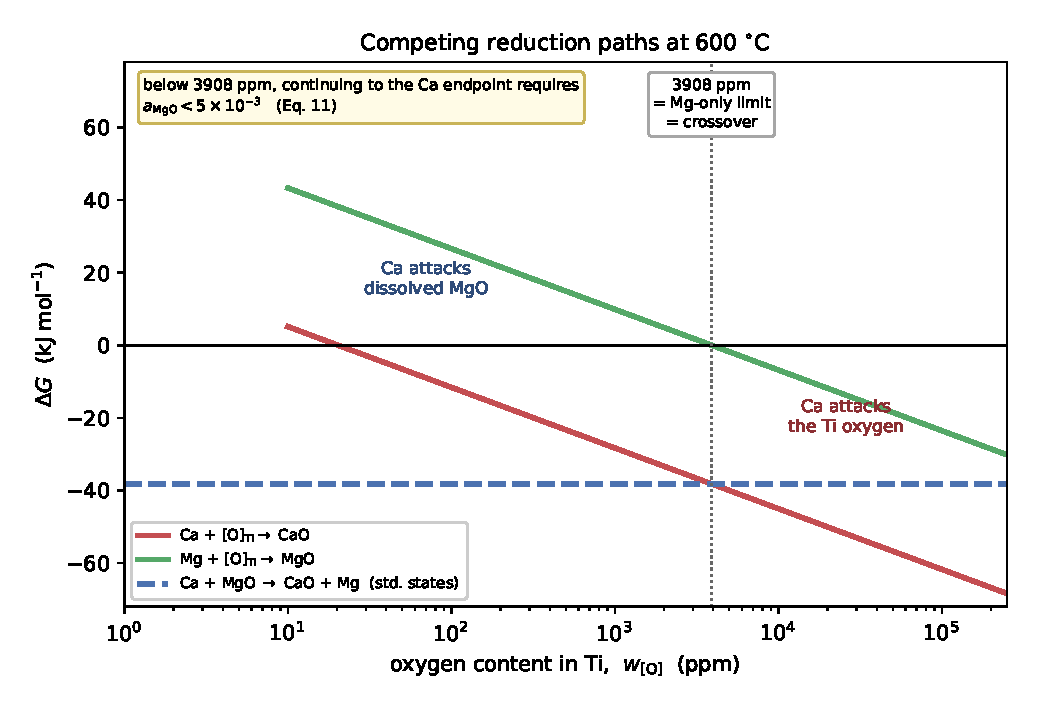
\includegraphics[width=0.80\linewidth]{figure_r3_competition.eps}
\caption{Competing reduction paths at 600~$^{\circ}$C. The driving forces of $\ce{Ca} + [\mathrm{O}]_{\mathrm{Ti}} \to \ce{CaO}$ (red) and $\ce{Mg} + [\mathrm{O}]_{\mathrm{Ti}} \to \ce{MgO}$ (green) both become more negative as the oxygen content rises, whereas that of the cross reaction $\ce{Ca + MgO -> CaO + Mg}$ (blue, standard states) is independent of it. The two curves cross the cross-reaction line at the same oxygen content, 3910~ppm---identically the Mg-only deoxidation limit of Eq.~\ref{eq:cross}---so below that value Ca preferentially consumes dissolved MgO unless $a_{\ce{MgO}} < 5\times10^{-3}$ (Eq.~\ref{eq:amgo}).}
\label{fig:competition}
\end{figure}

The alloy-state correction then applies as before: with $a_M = \gamma_{\mathrm{alloy}} x_M = 0.526 \times 0.5 = 0.263$, both endpoints rise by a factor of $\sim$3.8 ($\sim$14{,}900~ppm for Mg, $\sim$77~ppm for Ca), and the design-relevant deoxidation depth is the alloy-corrected Ca value of $\sim$77~ppm---still far below the 0.10--0.20~wt\% commercial target. The Mg rows of Table~\ref{tab:deox} are accordingly the endpoint of Mg acting alone, which by Eq.~\ref{eq:camgo} is simultaneously the crossover below which Ca begins to consume MgO, while the Ca rows give the design-relevant depth. Because $w_{[\mathrm{O}]} \propto 1/a_{\mathrm{M}}$, the depth is composition-dependent: in a Ca-dilute local region ($x_{\mathrm{Ca}} = 0.1$, $\gamma_{\mathrm{Ca(alloy)}} = 0.111$ from the full Redlich--Kister expansion rather than 0.125 from the regular-solution approximation, $a_{\mathrm{Ca}} = 0.0111$) the Ca endpoint rises to $\sim$1{,}800~ppm.

It should also be emphasized that $a_M = 0.263$ is a \emph{global} equimolar average; the cathode-surface alloy composition varies spatially and temporally, so the local equilibrium oxygen content is inhomogeneous. Which of the two limiting oxygen-transfer pictures applies---Mg and Ca each carrying roughly half of the oxygen (the 1:1 balance of Table~\ref{tab:mbalance}), or Ca acting as the sole net oxygen carrier---is decided by the competition between MgO dissolution and electrolytic regeneration on the one hand and its chemical reduction by the alloy at the alloy/salt interface on the other. That competition is kinetic rather than thermodynamic: the 1:1 material balance requires the electrolytic pathway to dominate, whereas if reaction~\ref{eq:camgo} is fast the regenerated species becomes CaO, the decomposition voltage rises from 2.73 to 2.83~V and the net energy consumption from 12{,}552 to 12{,}933~kWh/ton-Ti ($+$3\%; see the Material and Energy Balance section). Both limits lie below the FFC range, so the energy conclusion is unaffected either way. The interfacial kinetics of reaction~\ref{eq:camgo} are therefore identified as the critical unmeasured parameter of the proposed mechanism (Limitations~(10)).

\subsection*{Cathodic Co-Deposition and the Identity of the Net Oxygen Carrier}

Cathodic co-deposition and the identity of the net oxygen carrier are two distinct questions, and the design depends on separating them. At the cathode, $\ce{Mg^{2+}}$ discharges first---its equilibrium potential is $\sim$816~mV more positive---and $\ce{Ca^{2+}}$ joins once Mg deposition reaches its mass-transfer limit (Fig.~\ref{fig:current_regimes}a), so the alloy is genuinely co-deposited; that co-deposition is what supplies a liquid reductant at 600~$^{\circ}$C, where both pure metals are solid. The roles are not symmetric in the reduction that follows. MgO formed by Mg reducing $\ce{TiO2}$ is thermodynamically unstable in the presence of Ca (Eq.~\ref{eq:camgo}), and because that reaction generates no solid barrier---CaO leaves the interface by dissolution and Mg returns to the alloy---no product layer retards it, so its rate should not be lower than that of the interfacial deoxygenation of $\ce{TiO2}$, which must proceed through a growing Ti layer. Under that condition Ca is the net oxygen carrier: oxygen enters the melt as dissolved CaO and is evolved at the anode, while Mg shuttles oxygen between the particle surface and the dissolved Ca with no net chemical consumption (Table~\ref{tab:mbalance}, note~a).

The opposite limit---MgO dissolving and being regenerated electrolytically, so that Mg and Ca each carry about half of the oxygen---remains the bounding case and is retained because the interfacial rate of Eq.~\ref{eq:camgo} has not been measured. The two limits differ by 3\% in net energy (12{,}933 versus 12{,}552~kWh/ton-Ti), so no conclusion of this work depends on which applies. The CaO-only case is identified as the mechanistically favoured steady state, while the 1:1 balance is retained as the conservative design basis, crediting the cell with two electrolytic regeneration paths and therefore imposing the more demanding assumption on the energy balance. What the title's ``co-deposition'' refers to is the cathodic event, not a partition of the oxygen between the two metals.

\subsection*{Solid-State Deoxygenation and the Pore-Volume Constraint on \texorpdfstring{$a_{\ce{MgO}}$}{aMgO}}

Because $\ce{TiO2}$ is insoluble in the quaternary chloride melt, the reduction is not an electrochemical deposition of dissolved titanium ions but a solid-state deoxygenation at a liquid-metal/oxide interface. The reductant is delivered to the particle as a liquid Mg--Ca phase, oxygen is stripped from the oxide lattice as $\ce{O^{2-}}$ and transferred to the melt, and the metallic Ti remains in place, inheriting the external dimensions of the precursor while developing an internal pore network. Two consequences follow. First, the product is necessarily a porous powder rather than a dense deposit, which is why recovery is a powder-handling problem (see the Product recovery paragraph above). Second, the rate-limiting step is interfacial deoxygenation coupled to transport through the product layer---the quantity the SCM analysis models---rather than solution-phase mass transfer, which is also why the FFC analogy for current efficiency applies to the electrolysis step only and not to the reduction step.

The same picture supplies an independent, geometric justification for the $a_{\ce{MgO}} \lesssim 5\times10^{-3}$ requirement of Eq.~\ref{eq:amgo}. Per mole of Ti the solid volumes are 18.9~cm$^3$ ($\ce{TiO2}$), 10.6~cm$^3$ (Ti) and 22.5~cm$^3$ (2~mol MgO): were the MgO formed by Mg reduction retained as a solid within the particle, the solid volume would grow by $\approx$75\%, and the pore network that admits the liquid reductant would be filled long before the reaction reached the core. The designed route avoids this not by preventing MgO formation---which the thermodynamics of Eq.~\ref{eq:camgo} do not permit---but by keeping the dissolved MgO activity low enough that MgO leaves the reaction zone as it forms. The geometric and the thermodynamic bounds therefore coincide and point to the same requirement: the MgO removal rate, by dissolution and electrolytic regeneration, must match its formation rate.

The temperature-dependent dissolution free energy $\Delta G^{\circ}_{\mathrm{diss}} \approx -581{,}000 + 92T$~J/mol is derived from the CALPHAD assessment of the Ti--O system \cite{waldner1999}, which is validated for the $\alpha$-Ti phase field ($<$882~$^{\circ}$C). Across the operating window of 580--650~$^{\circ}$C the equilibrium oxygen content shifts by roughly $\sim$30\% (Mg) to a factor of $\sim$2 (Ca) (Table~\ref{tab:deox}); because Ca remains $\sim$100$\times$ deeper than Mg throughout this window, the order-of-magnitude conclusion is unaffected.

\begin{table}[!ht]
\centering
\footnotesize
\caption{Equilibrium oxygen content in titanium. Columns ``$a_M=1$'' assume pure metal; columns ``$a_M=0.263$'' account for the Mg--Ca liquid alloy activity ($\gamma_{\mathrm{alloy}}=0.526$, $x_M=0.5$). The Mg rows give the endpoint of Mg acting alone and, because Ca reduces MgO (Eq.~\ref{eq:camgo}), also the oxygen content below which Ca begins to consume dissolved MgO; the Ca rows give the design-relevant deoxidation depth, subject to $a_{\ce{MgO}} \lesssim 5\times10^{-3}$ (Eq.~\ref{eq:amgo}).}
\label{tab:deox}
\begin{tabular}{lccccc}
\toprule
Deoxidant/T & $\Delta G^{\circ}_{\mathrm{deox}}$ & $w_{[\mathrm{O}]}^{\mathrm{eq}}$ & $w_{[\mathrm{O}]}^{\mathrm{eq}}$ & $w_{[\mathrm{O}]}^{\mathrm{eq}}$ & $w_{[\mathrm{O}]}^{\mathrm{eq}}$ \\
 & (kJ/mol) & \multicolumn{2}{c}{$a_M=1$ (pure)} & \multicolumn{2}{c}{$a_M=0.263$ (alloy)} \\
\cmidrule(lr){3-4} \cmidrule(lr){5-6}
 & & (wt\%) & (ppm) & (wt\%) & (ppm) \\
\midrule
Mg / 550~$^{\circ}$C & $-7.5$ & 0.333 & 3325 & 1.264 & 12643 \\
Mg / 600~$^{\circ}$C & $-6.8$ & 0.391 & 3908 & 1.486 & 14859 \\
Mg / 650~$^{\circ}$C & $-6.1$ & 0.451 & 4510 & 1.715 & 17146 \\
Ca / 550~$^{\circ}$C & $-45.4$ & 0.0013 & 13.2 & 0.0050 & 50.2 \\
Ca / 600~$^{\circ}$C & $-45.0$ & 0.0020 & 20.2 & 0.0077 & 76.8 \\
Ca / 650~$^{\circ}$C & $-44.7$ & 0.0029 & 29.4 & 0.0112 & 111.8 \\
\bottomrule
\end{tabular}
\end{table}

\subsection*{\texorpdfstring{$\ce{Ca^{2+}/Na+}$}{Ca2+/Na+} Co-Deposition Window}

Table~\ref{tab:Ed} lists the standard decomposition voltages ($E_d$) and the corresponding reduction potentials ($E^{\circ}_{\mathrm{red}} = -E_d$) of the four pure chlorides at 600~$^{\circ}$C, all referenced to the $\ce{Cl2/Cl-}$ electrode.

\begin{table}[!ht]
\centering
\footnotesize
\caption{Decomposition voltages and reduction potentials of pure chlorides at 600~$^{\circ}$C (vs.\ $\ce{Cl2/Cl-}$). Note: $n$ denotes the number of electrons transferred per formula unit ($n = z_{\mathrm{cation}}$); $\Delta G^{\circ}_f$ values are Kirchhoff-corrected to 873~K from Barin \cite{barin1995}; $E_d = -\Delta G^{\circ}_f/(nF)$. Standard states are the pure solid salts (all four $T_m > 873$~K); on a liquid-reference activity basis each $E_d$ would increase by the melting free-energy term, shifting the Ca/Na window by $\approx$+30~mV and reinforcing the positive-window conclusion.}
\label{tab:Ed}
\begin{tabular}{lccc}
\toprule
Chloride & $\Delta G^{\circ}_f$ (kJ/mol) & $E_d$ (V) & $E^{\circ}_{\mathrm{red}}$ (V) \\
\midrule
$\ce{MgCl2}$ & $-501.9$ & 2.601 & $-2.601$ \\
$\ce{NaCl}$  & $-331.9$ & 3.440 & $-3.440$ \\
$\ce{CaCl2}$ & $-661.5$ & 3.428 & $-3.428$ \\
$\ce{KCl}$   & $-354.6$ & 3.675 & $-3.675$ \\
\bottomrule
\end{tabular}
\end{table}

Among the pure salts, $\ce{Mg^{2+}}$ is the easiest to reduce ($E^{\circ}_{\mathrm{red}} = -2.601$~V), while $\ce{K+}$ is the hardest ($-3.675$~V). Critically, $\ce{Ca^{2+}}$ and $\ce{Na+}$ have nearly identical reduction potentials in pure salts: $E^{\circ}_{\mathrm{red}}(\ce{Ca^{2+}/Ca}) - E^{\circ}_{\mathrm{red}}(\ce{Na+/Na}) = +12$~mV, meaning $\ce{Ca^{2+}}$ is marginally easier to reduce in pure salts. This $\pm$12~mV gap is within the $\approx\pm$2~kJ/mol uncertainty of the underlying $\Delta G^{\circ}_f$ data (see Data Sources and Computational Methods), which translates to $\approx\pm$20~mV for a monovalent chloride; the intrinsic Ca/Na preference is therefore weak, and the practical co-deposition selectivity is dominated by the concentration ratio ($x_{\ce{CaCl2}}/x_{\ce{NaCl}} = 0.40/0.15$) rather than by the intrinsic potential difference. The Downs process operates with a $\ce{CaCl2}$-majority electrolyte ($\sim$67~wt\% $\ce{CaCl2}$ / 33~wt\% $\ce{NaCl}$, roughly equimolar on a molar basis), yet deposits Na, because $\ce{Ca^{2+}}$ reduction is kinetically inhibited (large activation overpotential) relative to $\ce{Na+}$. The pure-salt near-identical potentials thus bear only superficial similarity to the Downs process: the Downs selectivity is \emph{kinetic} in origin, whereas the present $\ce{CaCl2}$-rich composition ($x_{\ce{CaCl2}}/x_{\ce{NaCl}} = 0.40/0.15$) adds a $\sim$120~mV \emph{thermodynamic} bias favoring Ca.

In the recommended quaternary composition ($x_{\ce{MgCl2}}=0.30$, $x_{\ce{CaCl2}}=0.40$, $x_{\ce{NaCl}}=0.15$, $x_{\ce{KCl}}=0.15$), Nernst concentration correction shifts the effective reduction potentials. The Nernst-corrected window $\Delta E = E_{\mathrm{red}}(\ce{Ca^{2+}}) - E_{\mathrm{red}}(\ce{Na+})$ becomes +120.2~mV under the ideal solution assumption (calculated using the $E^{\circ}_{\mathrm{red}}$ values from Table~\ref{tab:Ed} at 600~$^{\circ}$C), meaning $\ce{Ca^{2+}}$ now reduces before $\ce{Na+}$. As shown by the activity-coefficient sensitivity analysis, the window remains positive (74.9--147.1~mV) across all 18 tested $\gamma$ combinations ($\gamma_{\ce{CaCl2}} = 0.3$--1.0), suggesting the robustness of the composition design.

The above window is an \emph{equilibrium} quantity. Under polarization the effective deposition potentials shift by the activation overpotential $\eta_{\mathrm{act}} = (RT/\alpha nF)\,\mathrm{asinh}(j/2j_0)$. Adopting order-of-magnitude values typical of chloride melts ($j_0^{\mathrm{Ca}}\approx 0.05$~A/cm$^2$, $j_0^{\mathrm{Na}}\approx 0.03$~A/cm$^2$, $\alpha = 0.5$) \cite{pletcher1990}, the overpotential of monovalent $\ce{Na+}$ grows far faster than that of divalent $\ce{Ca^{2+}}$ (Fig.~\ref{fig:overpotential}): at $j = 0.5$~A/cm$^2$, $\eta_{\mathrm{act}}^{\mathrm{Ca}} \approx 174$~mV versus $\eta_{\mathrm{act}}^{\mathrm{Na}} \approx 424$~mV, which would \emph{widen} the effective window from 120.2~mV to $\sim$370~mV. This estimate is qualitative and its sign is not established: the assumed $j_0^{\mathrm{Ca}} > j_0^{\mathrm{Na}}$ favours Ca, yet the Downs cell deposits Na from a $\ce{CaCl2}$-majority melt, indicating that $\ce{Ca^{2+}}$ reduction may instead be kinetically \emph{slower}, which would \emph{narrow} the practical window. The $j_0$ and $\alpha$ values for the quaternary melt are unknown and require cyclic-voltammetry measurement, so the direction of the kinetic correction must be established before the enlarged window of Fig.~\ref{fig:overpotential} can be relied upon; concentration polarization at very high $j$ could additionally reverse the trend by depleting $\ce{Ca^{2+}}$ at the cathode.

\begin{figure}[!ht]
\centering
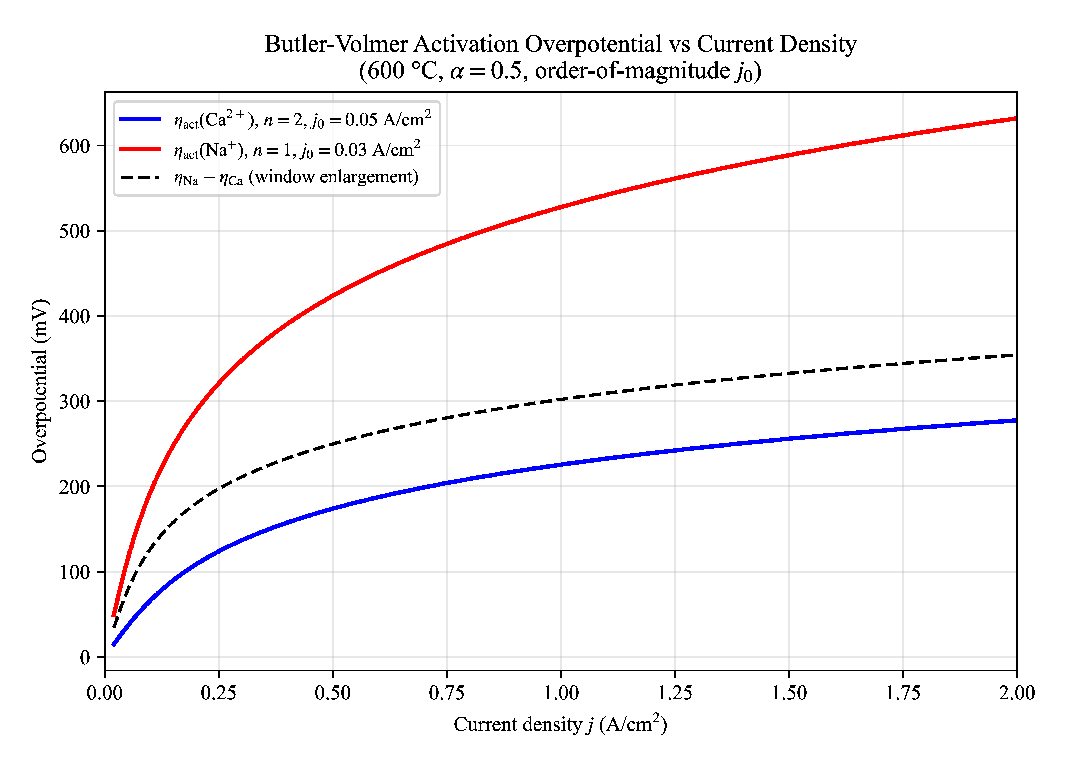
\includegraphics[width=0.85\linewidth]{figure2.eps}
\caption{Butler--Volmer activation overpotentials of $\ce{Ca^{2+}}$ ($n=2$) and $\ce{Na+}$ ($n=1$) versus current density at 600~$^{\circ}$C ($\alpha=0.5$, order-of-magnitude $j_0$). The dashed line is the kinetic enlargement of the co-deposition window, $\eta_{\mathrm{Na}} - \eta_{\mathrm{Ca}}$.}
\label{fig:overpotential}
\end{figure}

\emph{Mg/Ca co-deposition ratio.} The analysis above concerns only the $\ce{Ca^{2+}/Na+}$ selectivity. The far larger $\ce{Mg^{2+}/Ca^{2+}}$ gap is not addressed by the equilibrium window: at the recommended composition ($x_{\ce{MgCl2}}=0.30$, $x_{\ce{CaCl2}}=0.40$), the Nernst-corrected potentials give $E_{\mathrm{red}}(\ce{Ca^{2+}}) - E_{\mathrm{red}}(\ce{Mg^{2+}}) \approx -816$~mV, i.e., Mg reduces $\sim$816~mV earlier than Ca. The equimolar Mg--Ca alloy assumed in the Mg--Ca alloy thermodynamic analysis and in the material balance (Table~\ref{tab:mbalance}) is therefore \emph{not} a thermodynamic outcome: it can only be approached when Mg deposition reaches its mass-transfer (diffusion) limit at the cathode, after which Ca co-deposits, as in conventional alloy co-deposition (e.g., Zn--Ni, Li--Na). Mg--Ca co-deposition has in fact been demonstrated experimentally in $\ce{KCl-CaCl2-MgCl2}$ melts at 943~K, where bulk alloys comprising $\alpha$-Mg and $\ce{Mg2Ca}$ were obtained by galvanostatic electrolysis at 6~A/cm$^2$ \cite{tang2015}. The actual Mg/Ca ratio is thus set by the operating current density relative to the Mg limiting current density, as quantified in the following section, and the 1:1 assumption should be regarded as a bounding idealization.

\subsection*{Cathode Mass Transport and Operating Current Density}
\label{subsec:masstransport}

The qualitative argument above is made quantitative through a diffusion-layer analysis of the cathode. For each depositing cation, the limiting current density is
\begin{equation}
\label{eq:jlim}
j_{\mathrm{lim},i} = \frac{n F D_i\, c_{i,b}}{\delta}
\end{equation}
where $D_i$ is the melt-phase diffusivity, $c_{i,b}$ the bulk molar concentration, and $\delta$ the cathodic diffusion-layer thickness. The bulk concentrations follow from the melt density and composition: with $\rho \approx 1.8$~g/cm$^3$ and $M_{\mathrm{avg}} \approx 92.9$~g/mol at 600~$^{\circ}$C \cite{sato1999}, $c_{\mathrm{melt}} \approx 1.94\times10^{4}$~mol/m$^3$, giving $c_{\ce{MgCl2}} \approx 5.8\times10^{3}$~mol/m$^3$ and $c_{\ce{CaCl2}} \approx 7.8\times10^{3}$~mol/m$^3$ at the recommended composition. Taking $D = 1.0\times10^{-9}$~m$^2$/s---the conservative low end of the 1--3$\times10^{-9}$~m$^2$/s range measured in $\ce{CaCl2}$-based melts \cite{fray2000,yan2007}, adopted here for the melt-phase cation (a distinct quantity from the product-layer diffusivity used in the SCM analysis)---and $\delta = 200~\mu$m for an unstirred-to-mildly-agitated melt, Eq.~\ref{eq:jlim} gives $j_{\mathrm{lim,Mg}} = 0.56$~A/cm$^2$ and $j_{\mathrm{lim,Ca}} = 0.75$~A/cm$^2$. The physical basis of this $\delta$ value follows from the melt hydrodynamics: chloride melts near their liquidus have viscosities of order 1--3~mPa$\cdot$s, so with $\rho \approx 1.8$~g/cm$^3$ the Schmidt number is $Sc = \mu/(\rho D) \sim 10^{3}$, and natural-convection or mild-stirring correlations for centimeter-scale electrodes give $\mathrm{Sh} = L/\delta \sim 10$--$10^{2}$, placing $\delta$ in the $10^{2}$--$10^{3}$~$\mu$m range, consistent with the adopted 200~$\mu$m.

Figure~\ref{fig:current_regimes}a maps the resulting deposition regimes. In Regime~I ($j < j_{\mathrm{lim,Mg}}$), Mg deposits alone under activation control. In Regime~II ($j_{\mathrm{lim,Mg}} < j < j_{\mathrm{lim,Mg}} + j_{\mathrm{lim,Ca}} = 1.31$~A/cm$^2$), Mg deposition is mass-transfer-limited and the additional current is carried by $\ce{Ca^{2+}}$, so the Ca molar fraction of the deposit rises as
\begin{equation}
\label{eq:xca}
x_{\mathrm{Ca}} = 1 - \frac{j_{\mathrm{lim,Mg}}}{j}
\end{equation}
both metals being divalent, the charge and mole fractions coincide. The equimolar alloy of the material balance (Table~\ref{tab:mbalance}) is thus obtained at $j = 2\,j_{\mathrm{lim,Mg}} \approx 1.1$~A/cm$^2$---a concrete operating design point in place of the earlier bounding idealization. In Regime~III ($j > 1.31$~A/cm$^2$), $\ce{Na+}$ begins to co-deposit; the Ca fraction is then capped at 57\%, and the Na co-deposition loss mechanism (iii) of the current-efficiency budget is triggered. The 816~mV Mg/Ca equilibrium gap is consistent with this picture: the concentration overpotential required to deplete $\ce{Mg^{2+}}$ at the cathode surface, $\eta_{\mathrm{conc}} = (RT/2F)\ln(c_b/c_s)$, reaches 816~mV only at $c_s/c_b = 3.8\times10^{-10}$, i.e., Mg deposition becomes essentially fully diffusion-limited well before the potential is driven to the $\ce{Ca^{2+}/Ca}$ onset, which is precisely the condition under which Regime~II exists.

Because the deposit ratio is fixed by $j_{\mathrm{lim,Mg}}/j$ rather than by the melt composition, the equimolar design point also fixes the Mg:Ca ratio of the metal entering the alloy. Since Mg is chemically regenerated by Ca (Eq.~\ref{eq:camgo}) and therefore has no net chemical consumption, the continuously deposited Mg must have an outlet---evaporation (the Mg vapour pressure is $\approx$180~Pa at 600~$^{\circ}$C), entrainment in the product, or periodic alloy withdrawal---if it is not to accumulate in the alloy pool and raise $a_{\mathrm{Mg}}$ at the expense of $a_{\mathrm{Ca}}$. Lowering the $\ce{MgCl2}$ fraction reduces $j_{\mathrm{lim,Mg}}$ and shifts the deposit towards Ca (at $x_{\ce{MgCl2}} = 0.10$ the Mg share falls from 51\% to 17\%), at the cost of a higher liquidus. The corresponding $\ce{MgCl2}$ makeup stream is sized by these physical losses---freeboard evaporation, entrainment in the drained bed and a small inventory bleed---and not by the titanium production rate: in the CaO-only limit the net chemical consumption of Mg is zero (Table~\ref{tab:mbalance}, note a), since reaction~\ref{eq:camgo} restores it. This inventory balance is an additional design constraint that the present conceptual study does not resolve (Limitations~(10)). The two channels are sketched in Fig.~\ref{fig:shuttle}.

\begin{figure}[!ht]
\centering
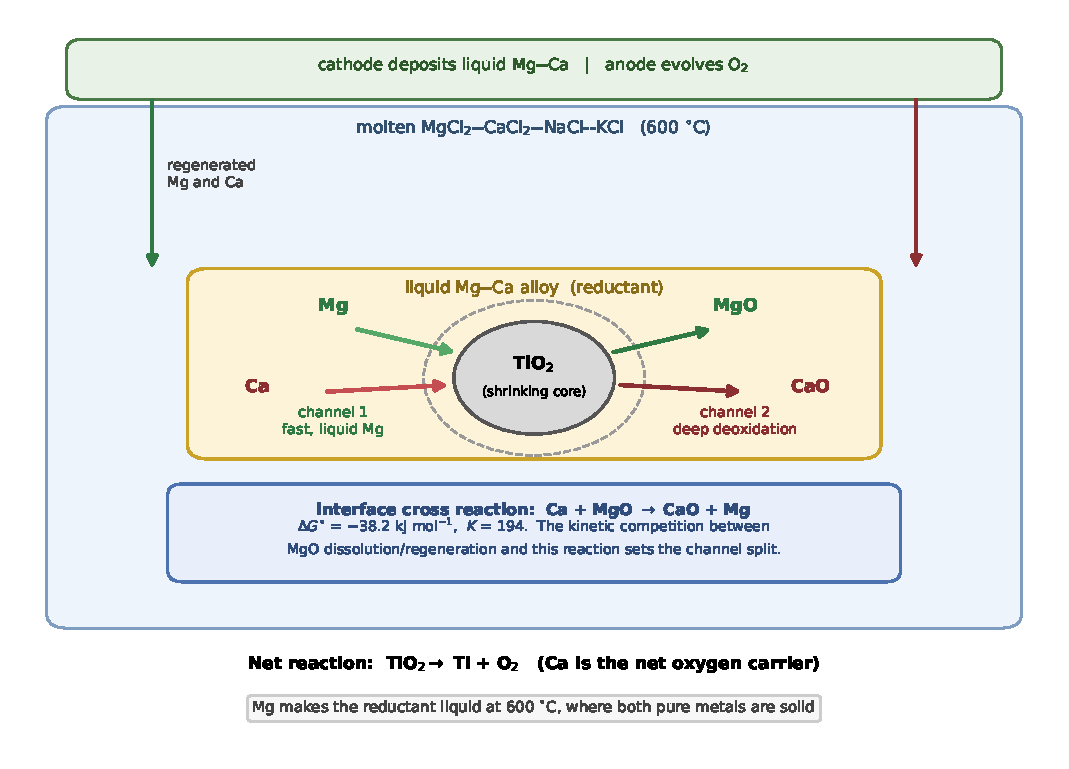
\includegraphics[width=0.82\linewidth]{figure_r3_shuttle.eps}
\caption{The two oxygen-transfer channels at a $\ce{TiO2}$ particle in contact with the liquid Mg--Ca alloy within the cathodic bed (schematic, not to scale). Channel~1: Mg reduces the particle, the MgO formed dissolves in the melt and is regenerated electrolytically. Channel~2: Ca reduces the particle and the residual oxygen, and the CaO formed is regenerated. At the alloy/melt interface the cross reaction $\ce{Ca + MgO -> CaO + Mg}$ (Eq.~\ref{eq:camgo}) returns Mg to the alloy; the steady-state split between the channels is set by the kinetics of that reaction relative to MgO dissolution and regeneration, the unmeasured quantity identified in Limitations~(10).}
\label{fig:shuttle}
\end{figure}

The analysis also fixes the cell-geometry constraint implicit in the ohmic term of the voltage budget (see the Material and Energy Balance section). With a representative melt conductivity $\kappa = 1.4$~S/cm \cite{sato1999}, the ohmic drop $jL/\kappa$ at $j \approx 1.1$~A/cm$^2$ is 0.40, 0.80, and 2.00~V for interelectrode gaps $L$ = 0.5, 1.0, and 2.5~cm, respectively (Fig.~\ref{fig:current_regimes}b). The 0.90~V ohmic budget allocated in the energy analysis therefore requires a melt path of $L \lesssim 1.1$~cm (tighter still once contact and busbar resistances are included), pointing to a close-spaced or diaphragm-integrated electrode configuration; at the 2.5~cm scale typical of many laboratory cells, the melt ohmic term alone would consume half of the 4.1~V cell voltage. At the design gap the anodic oxygen bubbles also occupy a small but non-negligible fraction of the interelectrode volume: the gas flux at $j = 1.1$~A/cm$^2$ corresponds to $\approx$2~mm/s of melt cross-section, so a 1.1~cm gap holds a void fraction of 1--2\% for bubble rise velocities of 0.1--0.2~m/s, and the Bruggeman correction $\kappa_{\mathrm{eff}} = \kappa(1-\varepsilon)^{3/2}$ lowers the effective conductivity by 1.5--3\%. The ohmic term therefore rises from 0.86 to 0.87--0.89~V, which remains inside the 0.90~V budget allocated in the energy analysis---not as a separately itemised loss, but as the margin between the nominal 0.86~V melt drop and the 0.90~V allocation.

Because $j_{\mathrm{lim}} \propto D/\delta$, the regime boundaries inherit the uncertainty of the transport parameters: over $D = 0.3$--$3\times10^{-9}$~m$^2$/s and $\delta = 100$--$500~\mu$m, $j_{\mathrm{lim,Mg}}$ spans 0.07--3.4~A/cm$^2$, an order of magnitude on either side of the nominal value. The operating current density must therefore be established for the actual melt---e.g., by cyclic voltammetry at a rotating or microelectrode---before the co-deposition design point can be fixed; the design framework (Eqs.~\ref{eq:jlim}--\ref{eq:xca}) then applies unchanged.

\begin{figure}[!ht]
\centering
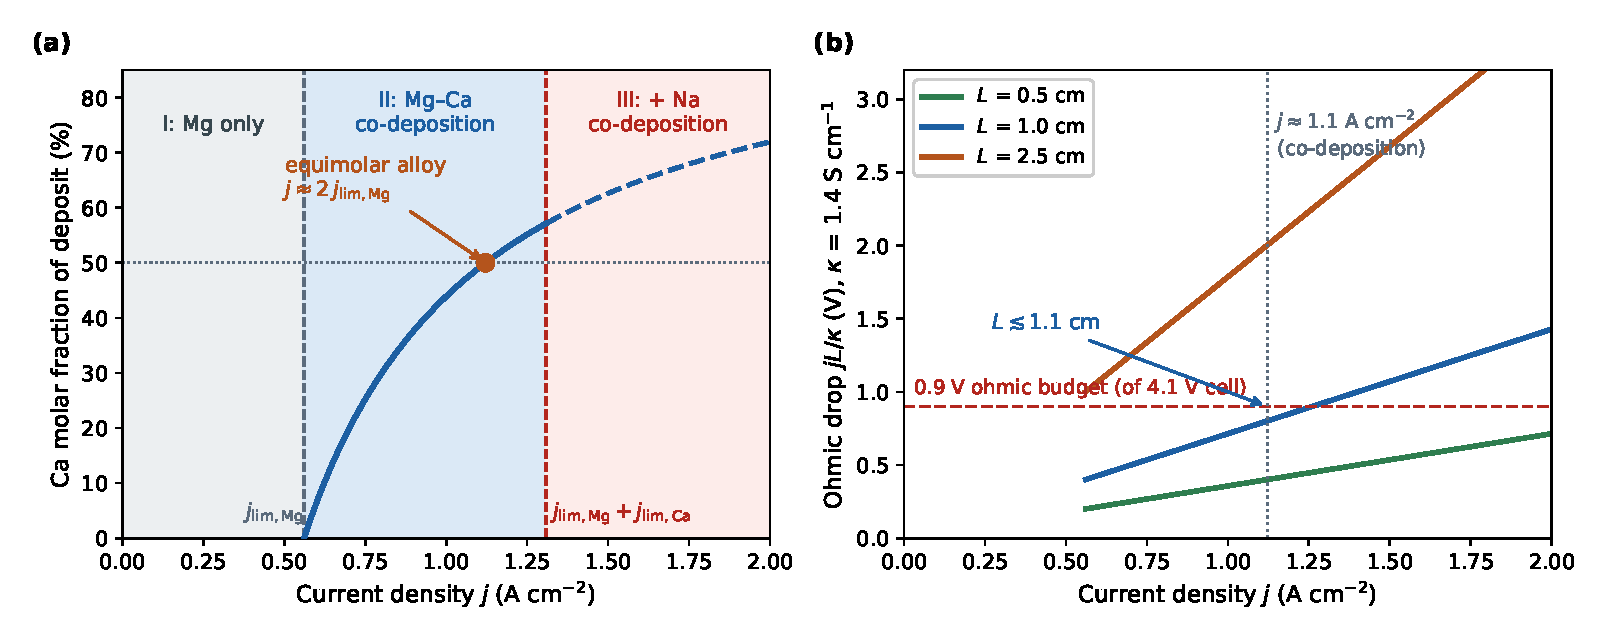
\includegraphics[width=0.95\linewidth]{figure3.eps}
\caption{Cathode co-deposition design map at 600~$^{\circ}$C ($D = 1.0\times10^{-9}$~m$^2$/s, $\delta = 200~\mu$m). (a) Deposition regimes versus current density: Regime~I, Mg only; Regime~II, Mg--Ca co-deposition with Mg at its limiting current and the Ca fraction given by Eq.~\ref{eq:xca} (solid), extrapolated beyond the Na$^+$ onset (dashed); Regime~III, Na$^+$ co-deposition onset. The marked point is the equimolar-alloy design point $j = 2\,j_{\mathrm{lim,Mg}} \approx 1.1$~A/cm$^2$. (b) Ohmic drop $jL/\kappa$ versus current density for interelectrode gaps $L$ = 0.5, 1.0, and 2.5~cm at $\kappa = 1.4$~S/cm; the 0.9~V budget requires $L \lesssim 1.1$~cm.}
\label{fig:current_regimes}
\end{figure}

\subsection*{\texorpdfstring{E--$p\ce{O^{2-}}$}{E-pO2-} Stability Diagram and Impurity Separation}

The E--$p\ce{O^{2-}}$ (Pourbaix-type) diagram for fused chloride systems \cite{littlewood1962} (Fig.~\ref{fig:EpO2}) plots the M/MO equilibrium lines according to:
\begin{equation}
\label{eq:epo2}
E = E^{\circ}_{\mathrm{red}} + \frac{RT}{2F}\ln(10)\cdot p\ce{O^{2-}}
\end{equation}
where $p\ce{O^{2-}} = -\log_{10}(a_{\ce{O^{2-}}})$ and $E^{\circ}_{\mathrm{red}} = \Delta G^{\circ}_{f,\mathrm{MO}}/(nF)$ is the standard reduction potential referenced to the $\ce{O2/O^{2-}}$ couple ($p_{\ce{O2}}=1$~atm, $a_{\ce{O^{2-}}}=1$), with $n$ the number of electrons transferred per oxide formula unit ($n=2$ for $\ce{MgO}$ and $\ce{CaO}$, $n=4$ for $\ce{TiO2}$ and $\ce{SiO2}$, $n=6$ for $\ce{Fe2O3}$ and $\ce{Al2O3}$). The derivation proceeds as follows: for a divalent-oxide half-reaction $\ce{MO + 2e^- -> M + O^{2-}}$, the Nernst equation gives $E = E^{\circ}_{\mathrm{red}} - (RT/2F)\ln(a_{\ce{O^{2-}}})$; substituting $\ln(a_{\ce{O^{2-}}}) = -\ln(10)\cdot p\ce{O^{2-}}$ yields the above equation with a positive slope. The slope is universal for all oxides: for a higher oxide such as $\ce{TiO2 + 4e^- -> Ti + 2O^{2-}}$, each $\ce{O^{2-}}$ exchanged still carries two electrons, so the coefficient of $p\ce{O^{2-}}$ remains $RT/2F$ and the stoichiometry enters only the intercept through $n$ in $E^{\circ}_{\mathrm{red}}$. All M/MO lines in Fig.~\ref{fig:EpO2} are therefore parallel, with the common slope of 86.6~mV per $p\ce{O^{2-}}$ unit at 600~$^{\circ}$C.

\begin{figure}[!ht]
\centering
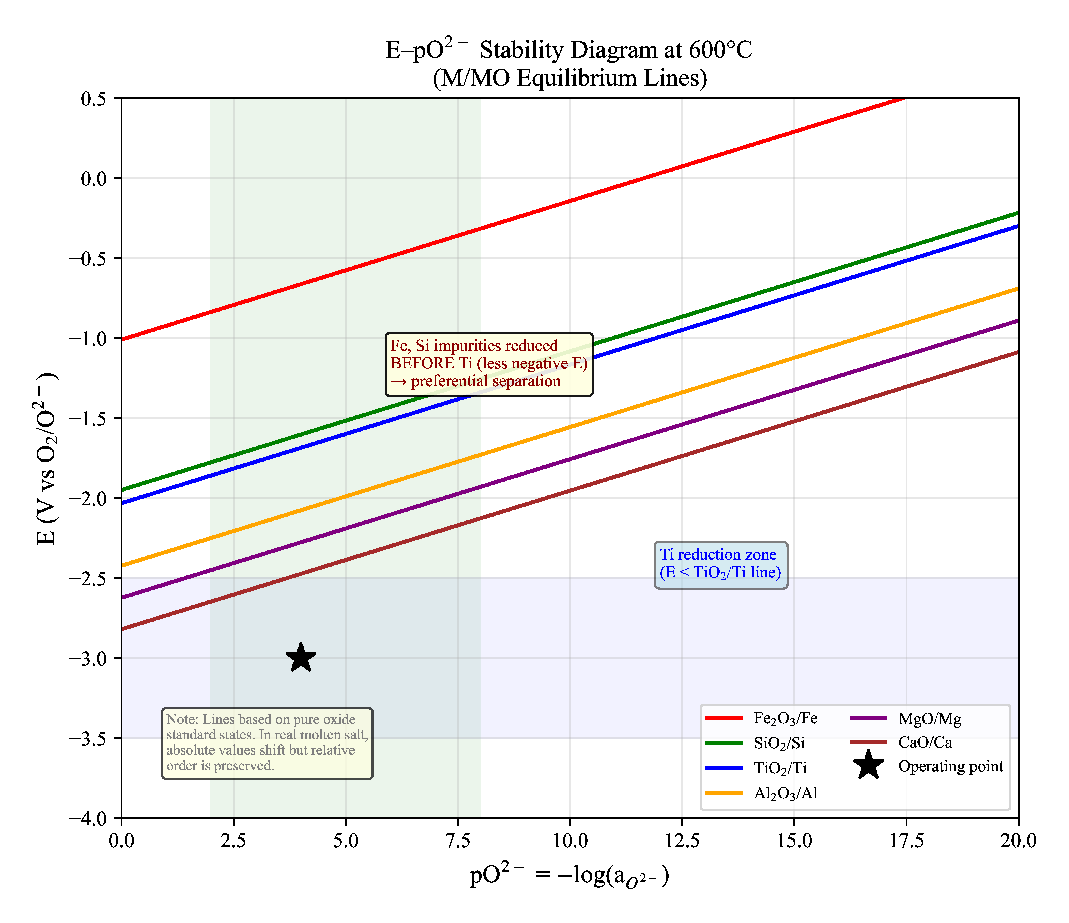
\includegraphics[width=0.95\linewidth]{figure4.eps}
\caption{E--$p\ce{O^{2-}}$ stability diagram at 600~$^{\circ}$C. All potentials are referenced to the $\ce{O2/O^{2-}}$ electrode ($p_{\ce{O2}}=1$~atm, $a_{\ce{O^{2-}}}=1$), not the $\ce{Cl2/Cl-}$ electrode used in Table~\ref{tab:Ed}. Lines based on pure oxide standard states; in real molten salt, $\ce{Ca^{2+}}$--$\ce{O^{2-}}$ complexation lowers $a_{\ce{O^{2-}}}$, shifting all potentials positively, but the relative reduction order ($\ce{Fe2O3} > \ce{SiO2} > \ce{TiO2} > \ce{Al2O3} > \ce{MgO} > \ce{CaO}$) is preserved.}
\label{fig:EpO2}
\end{figure}

The reduction potentials follow: $\ce{Fe2O3}$ ($-1.01$~V) $>$ $\ce{SiO2}$ ($-1.95$~V) $>$ $\ce{TiO2}$ ($-2.03$~V) $>$ $\ce{Al2O3}$ ($-2.42$~V) $>$ $\ce{MgO}$ $>$ $\ce{CaO}$, indicating that Fe and Si impurities reduce before Ti. This thermodynamic preferential reduction, combined with density differences (Fe: 7.87~g/cm$^3$ vs.\ Ti: 4.51~g/cm$^3$), suggests a potential pathway for physical separation of impurity metals from titanium powder. However, it should be noted that the Fe--Ti and Si--Ti systems exhibit extensive solid solubility and form intermetallic compounds (e.g., FeTi, $\ce{Fe2Ti}$, $\ce{Ti5Si3}$, $\ce{TiSi2}$) at 600~$^{\circ}$C, which may complicate gravity-based separation. The use of metallurgical-grade $\ce{TiO2}$ ($\geq$90~wt\%) thus requires further investigation of impurity phase distribution and may need complementary separation strategies (e.g., acid leaching). This thermodynamic basis indicates potential compatibility with metallurgical-grade $\ce{TiO2}$, subject to kinetic and purity validation. Notably, because $\ce{Ca^{2+}}$ exhibits stronger complexation with $\ce{O^{2-}}$ than $\ce{Mg^{2+}}$ does, the activity coefficient of dissolved CaO is suppressed more significantly than that of MgO. This differential non-ideality suggests that in a real chloride--oxide melt, the difference between CaO and MgO reduction potentials may be larger than predicted from pure-oxide standard states. Such a shift would be favorable for the proposed mechanism, reinforcing the division of labour adopted here: Ca provides the deoxidation depth, while the Mg--Ca alloy provides the liquid reductant phase and the transport path at the design temperature (see the Reduction Thermodynamics section).

\subsection*{SCM Kinetics and Parameter Sensitivity}
\label{subsec:scm}

\textbf{Model selection.} A shrinking-core formulation is adopted because the reduction proceeds by inward transport through a growing product layer around a shrinking unconverted core, which is the geometry of a solid--liquid reaction with a coherent product shell. The alternatives are less appropriate: pseudo-homogeneous (Avrami--Erofeev/JMAK) models assume reaction throughout the particle volume and describe nucleation-and-growth or gas--solid systems, whereas here the reductant is a liquid metal advancing from the particle surface inward; mixed-control formulations collapse to the shrinking-core result when internal diffusion through the product layer dominates, as argued below; and purely empirical rate laws would carry no predictive content for the $t \propto R^2$ particle-size scaling on which the process design depends. The weakest assumption of the model---diffusion control with a constant effective diffusivity---is examined below.

The reduction kinetics are modeled using the shrinking core model (SCM) with diffusion control through the porous Ti product layer \cite{levenspiel1999}:
\begin{equation}
\label{eq:scm}
t_{\mathrm{complete}} = \frac{c_{\mathrm{O}} \cdot R^2}{6\,D_{\mathrm{eff}}\,c_{\mathrm{red}}}
\end{equation}
where $c_{\mathrm{O}} \approx 1.06\times10^5$~mol/m$^3$ (oxygen concentration in $\ce{TiO2}$), $c_{\mathrm{red}} \approx 581$~mol/m$^3$ (3~mol\% dissolved Mg/Ca, from a melt density of 1.8~g/cm$^3$ \cite{sato1999} and $M_{\mathrm{avg}} \approx 92.9$~g/mol; dissolved-metal solubilities in the quaternary melt are not reported and single-salt values span 0.5--3~mol\%, so $t_{\mathrm{complete}} \propto 1/c_{\mathrm{red}}$ maps that range to 6.3--38~min), and $D_{\mathrm{eff}} = D\varepsilon/\tau$ with porosity $\varepsilon = 0.3$ and tortuosity $\tau = 3.0$ \cite{fray2000}. Here $D$ denotes the intrinsic diffusivity of the rate-limiting species through the porous Ti layer. Two mechanisms are possible---outward diffusion of O$^{2-}$ or inward diffusion of Mg/Ca---and $D = 2.0\times10^{-9}$~m$^2$/s is adopted as a representative value consistent with measured O$^{2-}$ diffusivities of 1--3$\times10^{-9}$~m$^2$/s in $\ce{CaCl2}$-based FFC melts \cite{fray2000,yan2007}; the range bounds either mechanism, so the nominal value does not presuppose which one controls. With these parameters, 100~$\mu$m particles ($R = 50~\mu$m) require 6.3~min for complete reduction (Fig.~\ref{fig:scm}).

\begin{figure}[!ht]
\centering
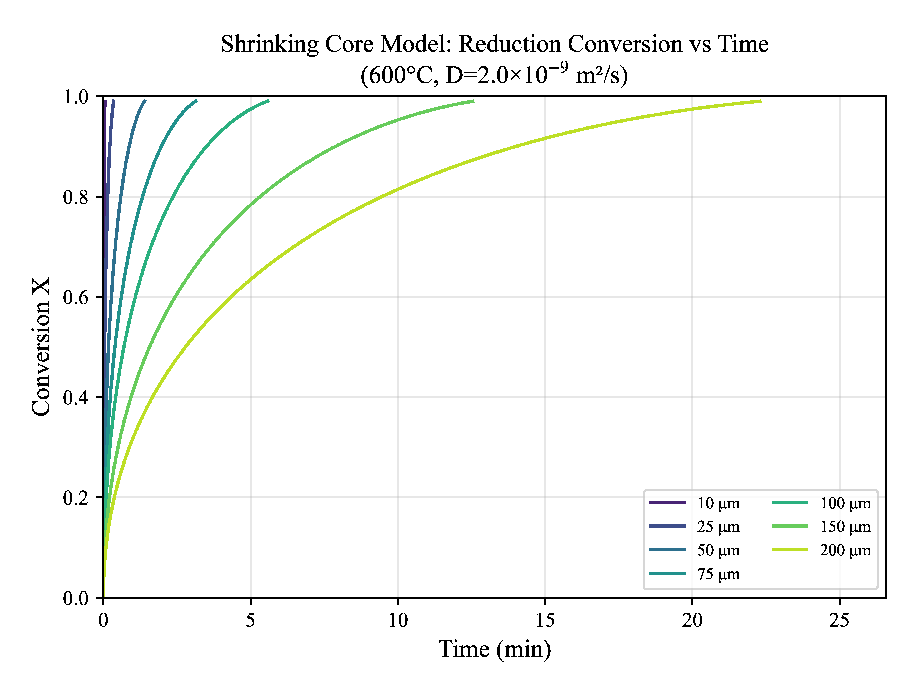
\includegraphics[width=0.95\linewidth]{figure5.eps}
\caption{SCM-predicted conversion versus time for different particle sizes ($D = 2.0\times10^{-9}$~m$^2$/s, 600~$^{\circ}$C).}
\label{fig:scm}
\end{figure}

A sensitivity analysis over $D = 1.0$--$3.0\times10^{-9}$~m$^2$/s (Fig.~\ref{fig:scm_sens}) shows that 100~$\mu$m-diameter particle reduction time ranges from 4.2~min ($D=3.0\times10^{-9}$) to 12.7~min ($D=1.0\times10^{-9}$), with the nominal 6.3~min falling within this range. The complete reduction time as a function of particle diameter is shown in Fig.~\ref{fig:scm_time}, illustrating the inverse-square scaling. Additional sensitivity to $\varepsilon$ (0.1--0.5) and $\tau$ (1.5--5.0) yields a broader $D_{\mathrm{eff}}$ range of $0.2\times10^{-10}$--$10\times10^{-10}$~m$^2$/s, corresponding to 1.3--63~min, indicating that precise prediction requires determination of product-layer microstructure.

The $D$ range of $10^{-9}$~m$^2$/s corresponds to liquid-phase diffusion through the pores of the product layer (Mg/Ca inward or O$^{2-}$ outward) and bounds either species. If the rate-limiting step were solid-state transport of O$^{2-}$ through the Ti layer, $D$ would be 2--3 orders of magnitude lower ($\sim$10$^{-12}$--10$^{-10}$~m$^2$/s) and 100~$\mu$m particles would require hours, making single-step batch reduction impractical; the process must therefore rely on the liquid-phase mechanism, which is plausible because the alloy is liquid at 600~$^{\circ}$C but requires experimental confirmation. External film diffusion can be neglected for 25--100~$\mu$m particles under mild agitation ($\mathrm{Sh} \gg 1$), although a quantitative comparison needs melt hydrodynamics that the conceptual stage does not provide.

To propagate uncertainties globally, a Monte Carlo simulation ($N = 10^5$, fixed random seed $= 42$ for reproducibility) sampled eleven parameters simultaneously. The first five are those of the energy and kinetic models: $D \sim U(1, 3) \times 10^{-9}$~m$^2$/s, $\varepsilon \sim U(0.1, 0.5)$, $\tau \sim U(1.5, 5.0)$, $\eta_I \sim \mathrm{Tri}(0.50, 0.75, 0.88)$, and $V_{\mathrm{cell}} \sim \mathcal{N}(4.1, 0.3)$ truncated to [3.5, 4.5]~V. Six further parameters cover the quantities that the earlier sensitivity discussion had left outside the sampling: $\gamma_{\ce{CaCl2}} \sim U(0.3, 1.0)$ and $\gamma_{\ce{NaCl}} \sim U(0.7, 1.0)$ (co-deposition window), the liquidus $T_{\mathrm{liq}} \sim \mathcal{N}(544, 25)$~$^{\circ}$C truncated to [494, 594]~$^{\circ}$C, the MgO solubility $S_{\ce{MgO}} \sim U(0.5, 1.2)$~wt\%, the diffusion-layer thickness $\delta \sim U(100, 500)$~$\mu$m, and the dissolved-reductant concentration $c_{\mathrm{red}} \sim U(0.5, 3.0)$~mol\%. The $\eta_I$ prior spans the worst-case FFC-like range without presupposing a feasibility threshold, and $\varepsilon$ and $\tau$ are sampled as independent uniform variables although they are physically negatively correlated, which makes the resulting $D_{\mathrm{eff}}$ spread conservative. In the energy calculation the cell voltage retains its nominal distribution, as in the energy balance; $\delta$ instead propagates into a \emph{design} consequence, because the equimolar deposit requires $j = 2j_{\mathrm{lim,Mg}}$ and the 0.9~V ohmic budget then fixes a required gap $L_{\mathrm{req}} = 0.9\kappa/j$.

The results (Fig.~\ref{fig:monte_carlo}) give a lognormal SCM reduction time with a median of 13.6~min (P5--P95: 4.0--55.2~min; the nominal 6.3~min corresponds to the upper end of the $c_{\mathrm{red}}$ range, 3~mol\%) and a right-skewed net energy consumption with a median of 13{,}141~kWh/ton-Ti (P5--P95: 10{,}875--16{,}722~kWh/ton-Ti) on the Case~II basis of Table~\ref{tab:mbalance}, and 13{,}536~kWh/ton-Ti on the CaO-only Case~I basis. The probability of beating the nominal 12{,}552~kWh/ton-Ti is 35.8\%, and $P(W_{\mathrm{net}} < 15{,}000) = 82.1\%$ (76.6\% for Case~I); the latter threshold is the lower bound of the FFC route, so that figure largely restates the assumed $\eta_I$ prior rather than providing an independent feasibility estimate. Spearman analysis (Fig.~\ref{fig:tornado}) shows that $\eta_I$ ($\rho = -0.85$) dominates the energy uncertainty ahead of $V_{\mathrm{cell}}$ ($\rho = 0.50$), while $c_{\mathrm{red}}$ and $\varepsilon$ dominate the SCM time, so experimental validation of current efficiency remains the most critical prerequisite for the energy claim. Because loss mechanisms (ii) and (iii) of the efficiency budget both scale with current density, a correlated variant of the same run was also evaluated, in which $\eta_I$ falls by 10\% per unit relative increase of $j$ above the nominal 1.1~A/cm$^2$: this raises the median net consumption from 13{,}141 to 13{,}981~kWh/ton-Ti and lowers $P(W_{\mathrm{net}} < 15{,}000)$ from 82.1\% to 65.9\%, showing that the energy claim is governed by the $\eta_I$--$j$ relation as much as by the efficiency value itself. $L_{\mathrm{req}}$ has a median of 0.84~cm and a 95th percentile of 1.88~cm, falling below a 3~mm engineering floor in only 4.2\% of the samples.

The added parameters act on \emph{feasibility} rather than on the per-ton energy (Fig.~\ref{fig:monte_carlo}c): the co-deposition window stays above the 50~mV threshold in every sample (5th percentile 89~mV), the ideal-solution liquidus is below 600~$^{\circ}$C throughout the sampled $\pm$50~$^{\circ}$C interval, and the joint probability that the window, the liquidus at the 620~$^{\circ}$C operating floor and the 3~mm gap floor are all satisfied is 95.8\%. Process feasibility is therefore not limited by any of these quantities individually, but by the two that cannot be computed at all---the 600~$^{\circ}$C CaO solubility and the Ca--MgO interfacial kinetics of Eq.~\ref{eq:camgo}.

\begin{figure}[!ht]
\centering
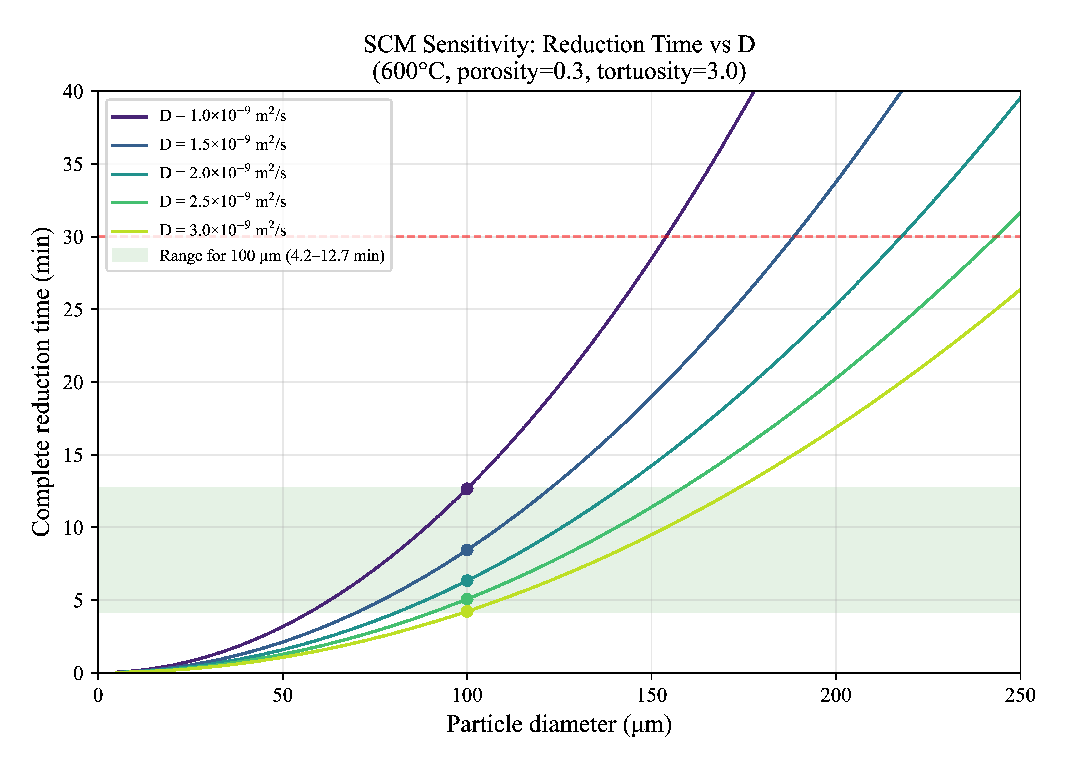
\includegraphics[width=0.95\linewidth]{figure6.eps}
\caption{SCM sensitivity analysis: reduction time versus particle diameter for $D = 1$--$3\times10^{-9}$~m$^2$/s.}
\label{fig:scm_sens}
\end{figure}

\begin{figure}[!ht]
\centering
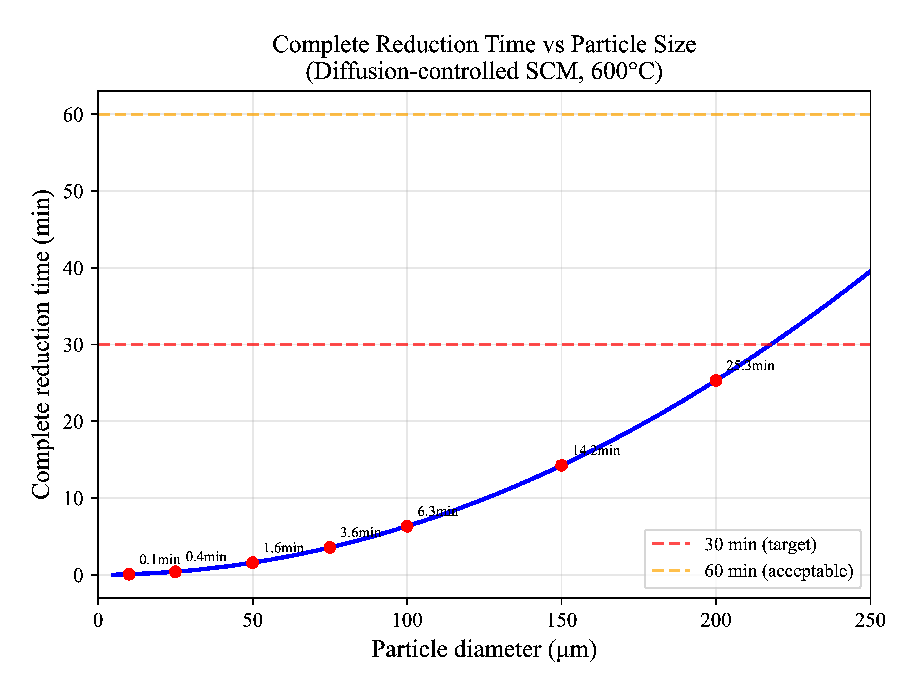
\includegraphics[width=0.95\linewidth]{figure7.eps}
\caption{Complete reduction time versus particle diameter at $D = 2.0\times10^{-9}$~m$^2$/s (600~$^{\circ}$C), showing the inverse-square scaling.}
\label{fig:scm_time}
\end{figure}

\begin{figure}[!htbp]
\centering
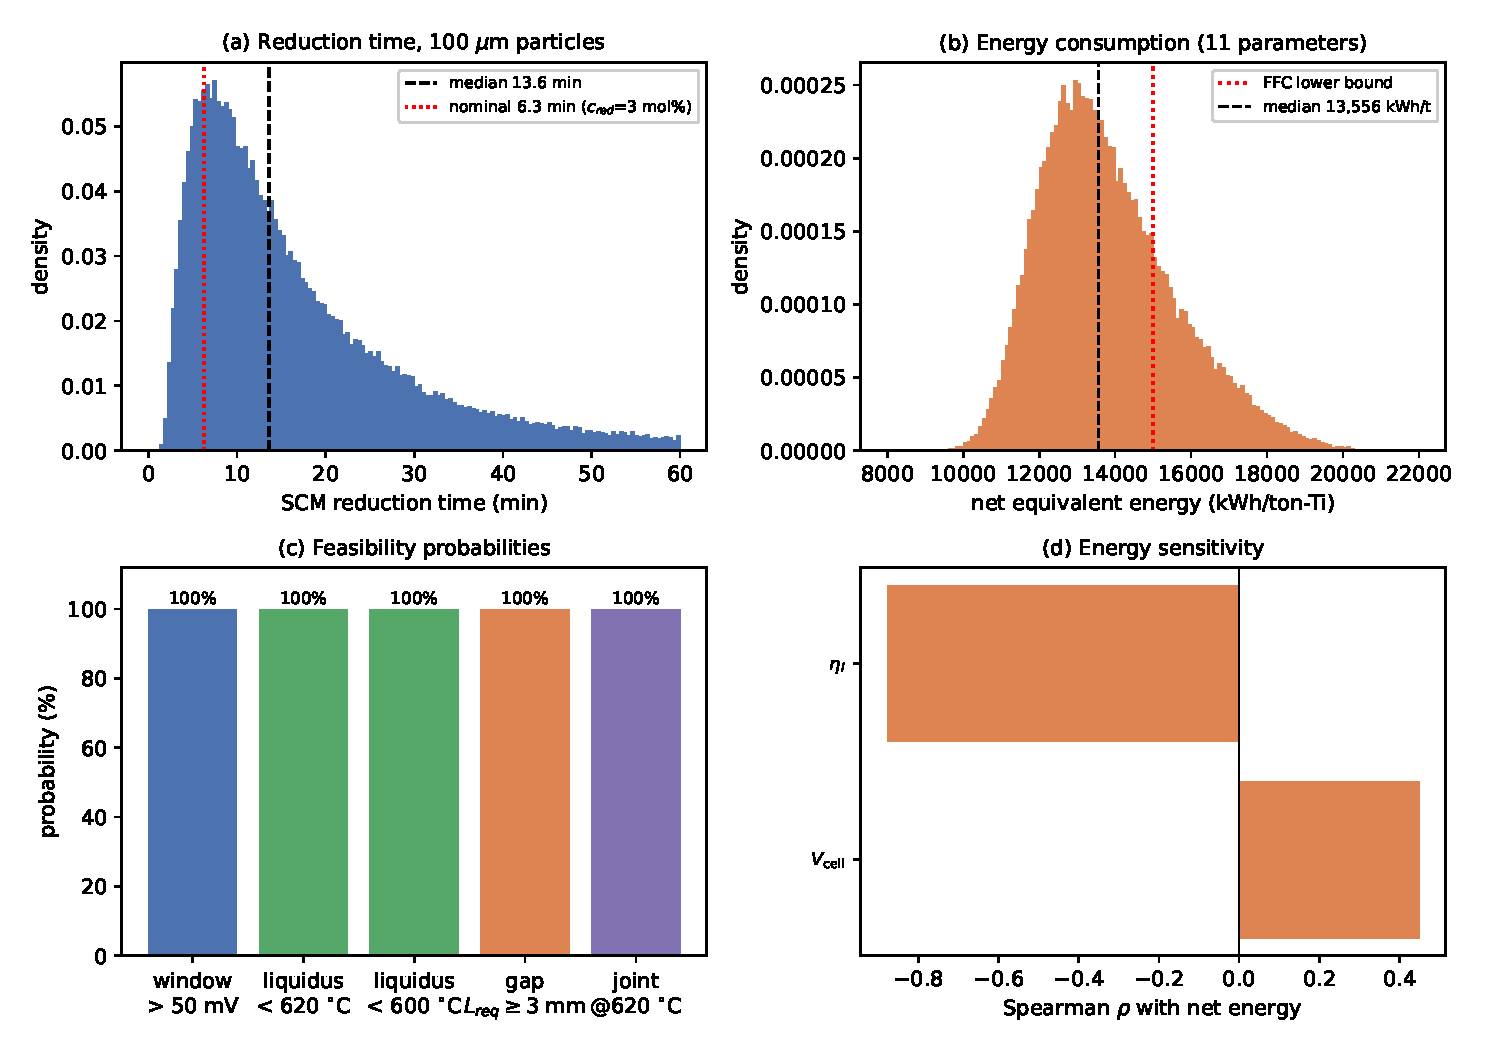
\includegraphics[width=0.95\linewidth]{figure8.eps}
\caption{Monte Carlo global uncertainty analysis ($N = 10^5$, eleven parameters): (a) SCM reduction time, with the nominal 6.3~min value marked (it corresponds to the upper end of the reductant-concentration range); (b) net energy consumption with the FFC lower bound; (c) probabilities that the co-deposition window exceeds 50~mV, that the liquidus lies below 600 and 620~$^{\circ}$C, and that the required interelectrode gap exceeds a 3~mm engineering floor, together with their joint probability at the 620~$^{\circ}$C operating floor; (d) Spearman rank correlation of each sampled parameter with the net energy. The sampled parameters are $D$, $\varepsilon$, $\tau$, $\eta_I \sim \mathrm{Tri}(0.50, 0.75, 0.88)$, $V_{\mathrm{cell}} \sim \mathcal{N}(4.1, 0.3)$, $\gamma_{\ce{CaCl2}}$, $\gamma_{\ce{NaCl}}$, the liquidus, the MgO solubility, the diffusion-layer thickness $\delta$ and the dissolved-reductant concentration $c_{\mathrm{red}}$.}
\label{fig:monte_carlo}
\end{figure}

\begin{figure}[!htbp]
\centering
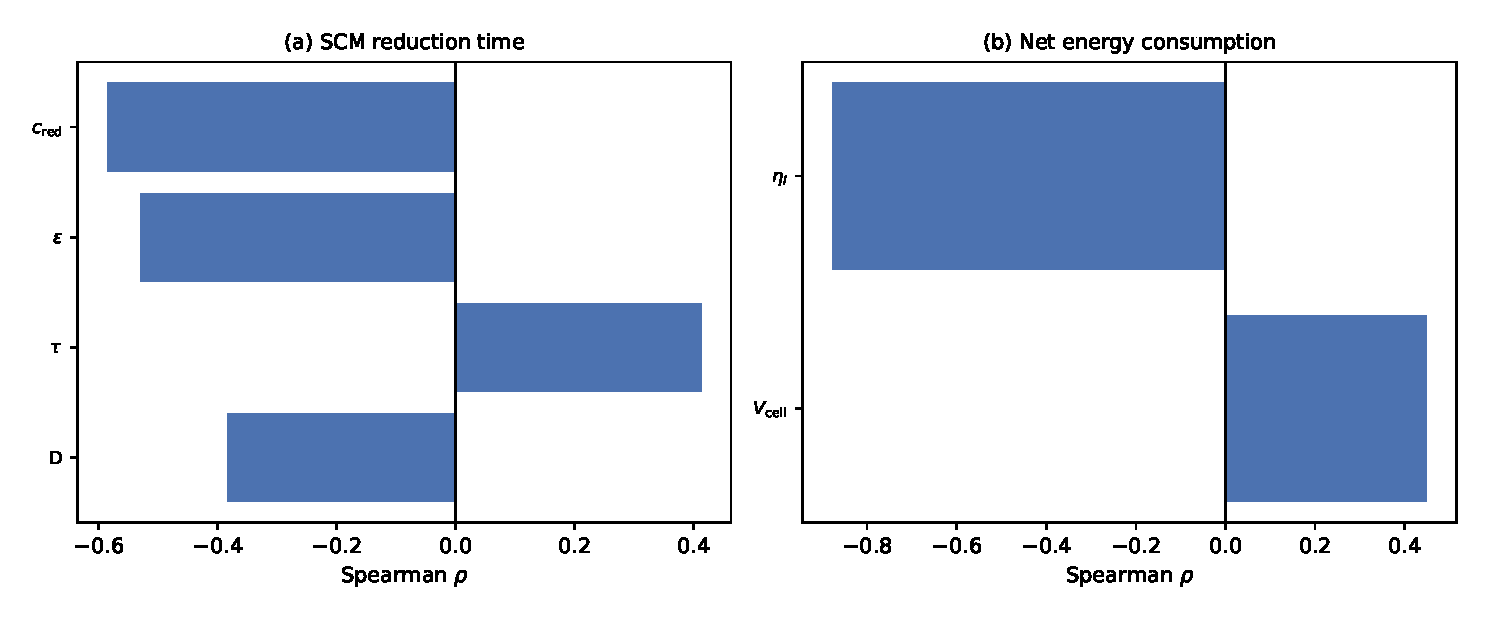
\includegraphics[width=0.95\linewidth]{figure9.eps}
\caption{Global parameter sensitivity (Spearman rank correlation) over the ten sampled parameters: (left) SCM reduction time; (right) net energy consumption.}
\label{fig:tornado}
\end{figure}

\subsection*{Material and Energy Balance}
\label{subsec:energy}

The material balance per ton Ti is split into two steps: (i) the chemical reduction step and (ii) the electrolytic regeneration step. In Step~(i), $\ce{TiO2}$ is reduced by Mg and Ca:
\begin{equation}
\ce{TiO2 + Mg + Ca -> Ti + MgO + CaO} \quad (3013~\mathrm{kg} = 3013~\mathrm{kg})
\end{equation}
In Step~(ii), the by-product oxides are electrolytically regenerated:
\begin{equation}
\ce{MgO + CaO -> Mg + Ca + O2} \quad (2013~\mathrm{kg} = 2013~\mathrm{kg})
\end{equation}
The net reaction is $\ce{TiO2 -> Ti + O2}$ ($1668~\mathrm{kg} = 1668~\mathrm{kg}$), with Mg and Ca acting as cyclic mediators. When using 90~wt\% metallurgical-grade $\ce{TiO2}$ ore, the impurity mass (186~kg/ton-Ti, mainly $\ce{Fe2O3}$ and $\ce{SiO2}$) enters as part of the ore input and exits as reduced impurity metals (Fe, Si), which require separation from the Ti product as discussed in the E--$p\ce{O^{2-}}$ stability diagram section.

\begin{table}[!ht]
\centering
\footnotesize
\caption{Material balance (basis: 1 ton Ti, pure $\ce{TiO2}$). Case~II is the design point used in this work, in which MgO and CaO are both regenerated electrolytically so that Mg and Ca each carry about half of the oxygen; Case~I is the limit in which Ca acts as the sole net oxygen carrier and the regenerated species is CaO (Eq.~\ref{eq:camgo}). The two cases differ only in which oxide is returned to the cell.}
\label{tab:mbalance}
\begin{tabular}{llcc}
\toprule
Category & Item & Case~II (kg) & Case~I (kg) \\
\midrule
Input & $\ce{TiO2}$ (pure) & 1668 & 1668 \\
 & Mg (cyclic) & 508 & $\le$1016 (net zero)$^{\mathrm{a}}$ \\
 & Ca (cyclic) & 837 & 1675 \\
\midrule
Output & Ti metal & 1000 & 1000 \\
 & $\ce{MgO}$ (to regeneration) & 842 & --- \\
 & $\ce{CaO}$ (to regeneration) & 1171 & 2343 \\
\midrule
Net & $\ce{TiO2} \to \ce{Ti} + \ce{O2}$ & \multicolumn{2}{c}{1668 = 1000 + 668} \\
\bottomrule
\end{tabular}

\par\footnotesize $^{\mathrm{a}}$In Case~I the Mg shuttles oxygen between the Ti particle surface and the Ca dissolved in the alloy---Mg is oxidised to MgO and chemically reduced back to Mg by Ca (Eq.~\ref{eq:camgo})---so its net chemical consumption is zero and only the amount needed to offset evaporation and entrainment must be replenished. The value quoted is the round-trip throughput, not a net consumption.
\end{table}

The theoretical decomposition voltage for simultaneous regeneration of MgO and CaO (4~e$^-$ per mol Ti) is 2.73~V, giving a theoretical minimum electrolysis energy of 6112~kWh/ton-Ti. In the CaO-only limit (Case~I of Table~\ref{tab:mbalance}) the corresponding values are $2\Delta G^{\circ}_{f}(\ce{CaO})/4F = 2.83$~V and 6334~kWh/ton-Ti. Because the charge transferred per mole of Ti is unchanged at 4~e$^-$, the only penalty of the CaO-only limit is the 99~mV higher decomposition voltage: the gross electrolysis demand rises from 12{,}244 to 12{,}625~kWh/ton-Ti and the net equivalent consumption from 12{,}552 to 12{,}933~kWh/ton-Ti ($+$3\%). Which case applies is decided by the kinetics of Eq.~\ref{eq:camgo} (Limitations~(10)); both are carried through this section so that the energy conclusion does not depend on that unresolved question. The assumed cell voltage ($\sim$4.1~V) is decomposed as $V_{\mathrm{cell}} = E_{\mathrm{decomp}} + \eta_{\mathrm{anode}} + \eta_{\mathrm{cathode}} + IR_{\mathrm{ohm}}$ (Fig.~\ref{fig:voltage_split}): the 2.73~V decomposition term is augmented by $\sim$0.30~V anode overpotential ($\ce{O2}$ evolution), $\sim$0.20~V cathode overpotential (Mg/Ca deposition), and $\sim$0.90~V ohmic drop (melt conductivity, contacts, busbars), summing to $\sim$4.13~V; the ohmic term is consistent with the interelectrode-gap constraint $L \lesssim 1.1$~cm at the co-deposition design current $j \approx 1.1$~A/cm$^2$ (Fig.~\ref{fig:current_regimes}b). These overpotential and ohmic terms are order-of-magnitude estimates, but they make explicit where the voltage---and hence the energy---is spent, and identify the anode overpotential and ohmic drop as the primary targets for cell design. Practical energy consumption depends on current efficiency $\eta_I$ and cell voltage $V_{\mathrm{cell}}$:
\begin{equation}
W_{\mathrm{practical}} = \frac{4F \cdot n_{\mathrm{Ti}} \cdot V_{\mathrm{cell}}}{\eta_I \cdot 3.6\times10^{6}}
\end{equation}

\begin{table}[!ht]
\centering
\footnotesize
\caption{Practical energy consumption (basis: 1 ton Ti)}
\label{tab:energy}
\begin{tabular}{cccl}
\toprule
$\eta_I$ & $V_{\mathrm{cell}}$ (V) & Energy (kWh/ton) & Condition \\
\midrule
0.85 & 3.5 & 9{,}222 & Best \\
0.80 & 4.0 & 11{,}198 & Moderate \\
0.75 & 4.0 & 11{,}944 & Conservative \\
0.75 & 4.3 & 12{,}840 & Graphite anode + ohmic \\
0.70 & 4.5 & 14{,}397 & Worst \\
\bottomrule
\end{tabular}
\end{table}

\begin{figure}[!ht]
\centering
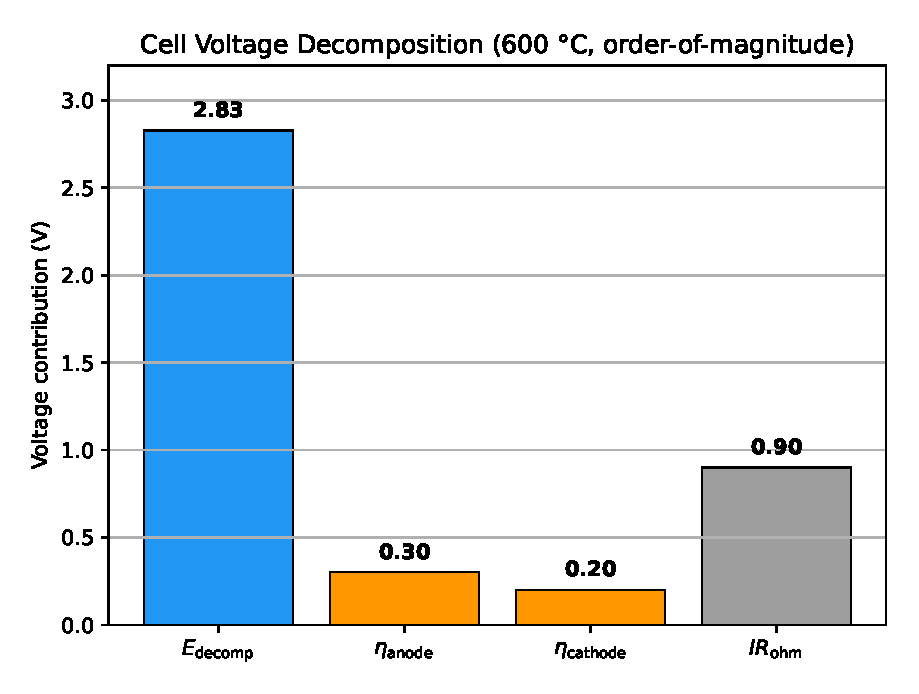
\includegraphics[width=0.7\linewidth]{figure10.eps}
\caption{Decomposition of the assumed cell voltage ($\sim$4.1~V) into the thermodynamic decomposition term (2.73~V), anode and cathode overpotentials, and ohmic drop (order-of-magnitude estimates).}
\label{fig:voltage_split}
\end{figure}

Under realistic conditions ($\eta_I = 0.75$--0.80, $V_{\mathrm{cell}} = 4.0$--4.3~V), the electrolysis-step energy consumption is 11{,}200--12{,}800~kWh/ton-Ti (Table~\ref{tab:energy}; electrolysis step only; full-process net consumption is 12{,}552~kWh/ton-Ti, see the Full-Process Energy Balance section). The sensitivity analysis (Fig.~\ref{fig:energy}) shows that $\eta_I \geq 74.7\%$ at $V = 4.0$~V is required to stay below 12{,}000~kWh/ton.

The assumed current efficiency range ($\eta_I = 0.75$--0.80) requires justification, as it significantly exceeds the FFC Cambridge process (30--50\%) \cite{fray2000}. The difference is mechanistic: FFC electro-deoxidises a solid oxide through a growing product layer, whereas the present process electrolyses dissolved oxides and therefore resembles dissolved-salt electrolysis---Hall--H\'eroult (90--95\% \cite{kvande2014}), Downs (70--90\%) and industrial $\ce{MgCl2}$ cells (80--90\% \cite{ji2026,pletcher1990}). The faradaic losses are estimated as (i) electronic conduction (2--5\%), (ii) back-dissolution of fresh Mg/Ca by dissolved oxide species (5--10\%), (iii) Na co-deposition at high $j$ (3--8\%) and (iv) impurity side reactions (2--5\%), summing to $\eta_I \approx 0.72$--0.88. A fifth channel is excluded from the faradaic budget because it conserves both metals: $\ce{Ca + Mg^{2+} -> Ca^{2+} + Mg}$ costs voltage efficiency rather than charge and caps the attainable deoxidation depth at the Mg-only endpoint (3908~ppm); its signature scales with the boundary-layer $\ce{Mg^{2+}}$ concentration and is separable from (ii) by comparing $\eta_I$ with the measured Ca:Mg ratio of the deposit. The estimates are additive and independent, and (ii) and (iii) both worsen with $j$, so the attainable $\eta_I$ at 1.1~A/cm$^2$ may fall below that sum; the Monte Carlo propagates $\eta_I$ independently and does not encode this correlation (Limitations~(9)). The target range is an \emph{unvalidated hypothesis}: at $\eta_I = 0.50$--0.60 the energy rises to $\sim$15{,}200--19{,}600~kWh/ton-Ti, within the FFC range, so the energy advantage is \emph{conditional on achieving $\eta_I > 0.70$}.

For context, the Kroll process consumes approximately 30{,}000--40{,}000~kWh/ton-Ti (industrial measured, including chlorination, Mg reduction, and vacuum distillation) \cite{ji2026}, while the FFC Cambridge process is estimated at 15{,}000--20{,}000~kWh/ton-Ti (pilot-scale measured, due to lower current efficiency of 30--50\% and higher operating temperature of $\sim$950~$^{\circ}$C) \cite{ji2026,fray2000}. The proposed process predicts 11{,}500--13{,}100~kWh/ton-Ti net equivalent consumption (\emph{theoretical prediction} based on assumed $\eta_I = 0.75$--0.80 and $V_{\mathrm{cell}} = 4.0$--4.3~V; electrolysis step alone 11{,}200--12{,}800~kWh/ton-Ti) primarily through reduced operating temperature (600~$^{\circ}$C), higher target current efficiency (75--80\%, conditional on achieving dissolved-oxide electrolysis performance comparable to Hall--H\'eroult and Downs processes), and elimination of the chlorination step. It should be emphasized that these are \emph{non-equivalent comparisons}: the proposed process values are theoretical predictions based on assumed parameters, while the Kroll and FFC figures are industrial/pilot-scale measured values with different system boundaries. A rigorous comparison requires unified cradle-to-gate boundary analysis.

A particularly relevant analogy is the Hall--H\'eroult process for aluminum production \cite{kvande2014}, which also electrolyzes a dissolved oxide ($\ce{Al2O3}$ in cryolite melt) rather than a solid cathode. Hall--H\'eroult achieves current efficiencies of 90--95\% at $\sim$950~$^{\circ}$C with DC energy consumption of $\sim$13{,}000~kWh/ton-Al and cell voltages of 4.0--4.2~V. The proposed Ti process shares the dissolved-oxide electrolysis mechanism but operates at significantly lower temperature (600~$^{\circ}$C), which reduces thermal losses and material corrosion. However, the higher decomposition voltage of $\ce{TiO2}$ (thermodynamic minimum $\sim$2.73~V vs.\ $\sim$2.2~V for $\ce{Al2O3}$, both on an O$_2$-evolving inert-anode basis) and the additional overpotentials for Mg/Ca co-deposition result in a higher cell voltage ($\sim$4.0--4.3~V). If the dissolved-oxide electrolysis mechanism can be confirmed experimentally, the Hall--H\'eroult analogy supports the feasibility of achieving $\eta_I > 0.70$, since the fundamental current-loss mechanisms (electronic conduction, back-reaction) are mitigated by the lower operating temperature and the chemical mediation via Mg/Ca cycling. The analogy is, however, limited to the electrolysis step: Hall--H\'eroult taps liquid aluminum directly from the metal pad, whereas the present process requires the co-deposited Mg--Ca alloy to contact and reduce the bed of settled $\ce{TiO2}$ particles---an additional liquid--solid reaction step (quantified by the SCM kinetics analysis) that aluminum electrolysis does not face.

\begin{figure}[!ht]
\centering
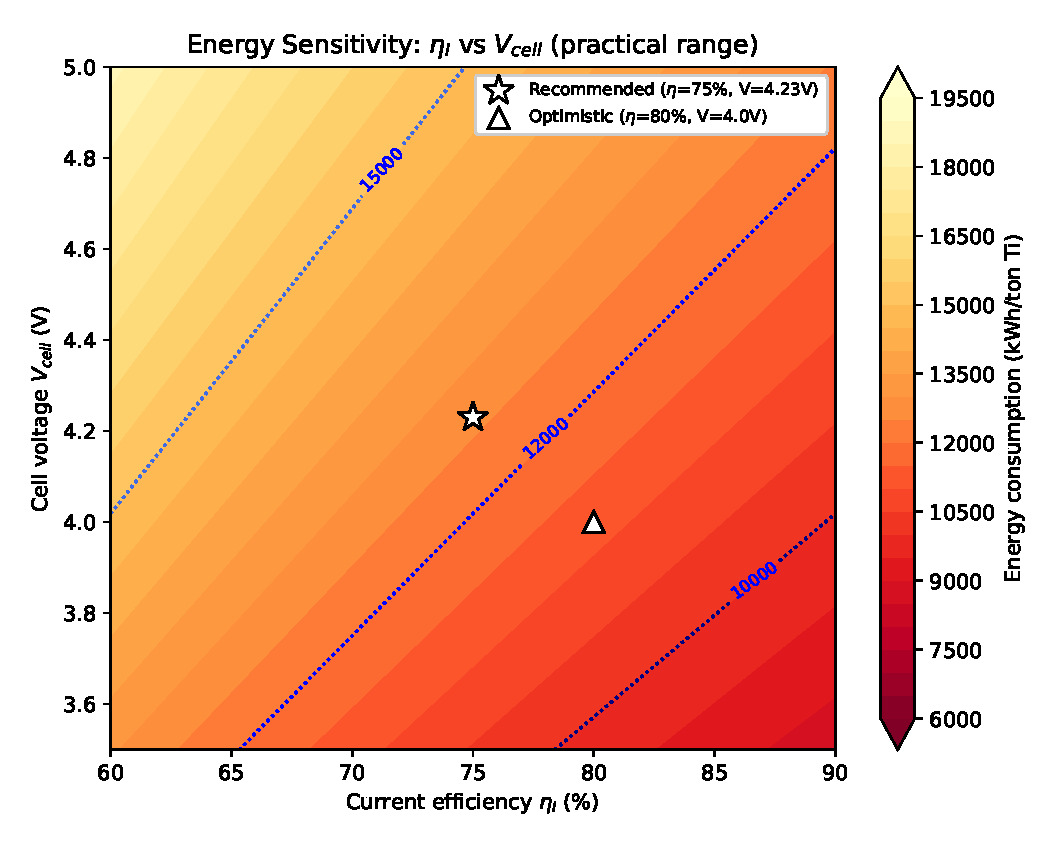
\includegraphics[width=0.95\linewidth]{figure11.eps}
\caption{Energy sensitivity: $\eta_I$ vs.\ $V_{\mathrm{cell}}$ (practical range; the electrolysis step minimum 6{,}112~kWh/ton and the net reaction reversible work $\sim$4{,}550~kWh/ton both lie below this range and are not shown).}
\label{fig:energy}
\end{figure}

\subsection*{Full-Process Energy Balance}
\label{subsec:heatbal}

The full-process energy balance (Table~\ref{tab:heatbal}), \emph{conditional on achieving $\eta_I > 0.70$} as discussed in the Material and Energy Balance section, is structured to distinguish electrical energy inputs from thermal effects. The electrolysis gross electrical demand is 12{,}244~kWh/ton ($\eta_I=0.75$, $V_{\mathrm{cell}}=4.1$~V), or 12{,}625~kWh/ton at $V_{\mathrm{cell}}\approx4.23$~V in the CaO-only Case~I of Table~\ref{tab:mbalance}. Because the cell voltage exceeds the thermoneutral voltage of the regeneration step ($\approx$3.20~V, from $\Delta H^{\circ}_{f}(\ce{MgO})+\Delta H^{\circ}_{f}(\ce{CaO}) = 1{,}236.7$~kJ per mole of Ti, i.e., per 4~e$^-$), the electrolysis cell is strongly self-heating: of the 12{,}244~kWh/ton electrical input, only $\approx$5{,}483~kWh/ton is absorbed as net reaction enthalpy and $\approx$6{,}761~kWh/ton must be rejected as waste heat, in addition to the 1{,}690~kWh/ton released by the exothermic reduction step (the two figures are consistent: the regeneration step absorbs $\approx$7{,}173~kWh/ton, which minus the 1{,}690~kWh/ton reduction exotherm gives the $\approx$5{,}483~kWh/ton net). The reduction exotherm therefore arises inside an already self-heating cell and is \emph{not} credited against electrical energy; it is treated as waste heat available for internal heat integration, offsetting at most the external thermal demand ($\ce{TiO2}$ preheating 184, salt makeup preheating 7, cell wall loss 138; total 329~kWh/ton). Auxiliary electrical inputs (salt circulation pumping 50, post-treatment 300) add 350~kWh/ton. With full heat integration, the net equivalent consumption is 12{,}244 + 350 $-$ 42 (Ti powder cooling recovery) $=$ 12{,}552~kWh/ton-Ti; without heat integration it is 12{,}881~kWh/ton-Ti.

\emph{Accounting note: thermal and electrical energy differ in quality (exergy). The heat-integration credit adopted above is capped at the 329~kWh/ton external thermal demand and requires no conversion of heat to work; no Carnot-limited work recovery from the $\sim$6{,}761~kWh/ton of rejected waste heat is credited.} The process energy efficiency---the ratio of the electrolysis step's theoretical minimum (6{,}112~kWh/ton) to the net equivalent external energy consumption (12{,}552~kWh/ton)---is 48.7\%, reflecting the combined irreversibilities of electrolysis (voltage efficiency $\approx$67\%, current efficiency 75--80\%) and thermal losses. The true second-law (exergetic) efficiency is lower: the net reaction $\ce{TiO2 -> Ti + O2}$ has a reversible work of $\sim$4{,}550~kWh/ton-Ti ($\Delta G^{\circ}_{\ce{TiO2}} \approx 783$~kJ/mol at 873~K), giving 36.3\%. The two differ because the electrolysis step must also regenerate the Mg/Ca mediators, whose decomposition energy exceeds the reversible work of the net reaction. The electrolysis energy fraction of 97.2\% indicates that electrolysis dominates the external energy budget; it is \emph{not} a thermodynamic efficiency.

\begin{table}[!ht]
\centering
\footnotesize
\caption{Full-process heat balance (basis: 1 ton Ti, 600~$^{\circ}$C). All values are for Case~II of Table~\ref{tab:mbalance}; in the CaO-only Case~I the thermoneutral voltage is 3.29~V, the gross electrical demand 12{,}625~kWh/ton, the regeneration enthalpy absorbed 7{,}369~kWh/ton (5{,}679 net of the 1{,}690~kWh/ton reduction exotherm), the heat rejected 6{,}946~kWh/ton, the net consumption 12{,}933~kWh/ton, the process efficiency 49.0\% (6334/12{,}933, each case evaluated against its own electrolysis minimum), the second-law efficiency 35.2\% and the electrolysis fraction 97.3\%.}
\label{tab:heatbal}
\begin{tabularx}{\linewidth}{l c X}
\toprule
Item & Energy (kWh/ton) & Note \\
\midrule
\multicolumn{3}{l}{\textit{Electrolysis}} \\
\quad Gross electrical demand & 12{,}244 & $W = 4F n_{\mathrm{Ti}} V_{\mathrm{cell}}/(\eta_I \cdot 3.6{\times}10^6)$ at $\eta_I=0.75$, $V_{\mathrm{cell}}=4.1$~V \\
\quad Reaction enthalpy absorbed (net) & $\approx$5{,}483 & $\Delta H = 944.7$~kJ/mol-Ti for $\ce{TiO2 -> Ti + O2}$; balance ($\approx$6{,}761) rejected as waste heat$^{\mathrm{a}}$ \\
\midrule
\multicolumn{3}{l}{\textit{Auxiliary inputs}} \\
\quad $\ce{TiO2}$ preheating & 184 & External thermal, met by reject-heat integration$^{\mathrm{a}}$ \\
\quad Salt makeup preheating & 7 & External thermal, met by reject-heat integration \\
\quad Cell wall heat loss & 138 & External thermal, met by reject-heat integration \\
\quad Salt circulation pumping & 50 & External input \\
\quad Post-treatment (washing/drying/screening) & 300 & External input (excludes impurity acid-leaching, see Limitations~(7)) \\
\midrule
\quad Total external input & 12{,}594 & Electricity 12{,}244 + pumping/post-treatment 350 (thermal needs met by integration) \\
\midrule
\multicolumn{3}{l}{\textit{Heat recovery}} \\
\quad Ti powder cooling (50\% recoverable) & $-$42 & External heat recovery \\
\midrule
\multicolumn{3}{l}{\textit{Net consumption}} \\
\quad Net energy & 12{,}552 & Total external input $-$ Ti cooling (12{,}881 without heat integration) \\
\quad Electrolysis step minimum & 6{,}112 & $\ce{MgO + CaO -> Mg + Ca + O2}$ at 873~K \\
\quad Net reaction reversible work & $\sim$4{,}550 & $\ce{TiO2 -> Ti + O2}$, $\Delta G^{\circ}\approx783$~kJ/mol at 873~K \\
\quad Process energy efficiency & 48.7\% & $6112/12552$ (equiv.) \\
\quad Second-law efficiency & $\sim$36.3\% & $4550/12552$ \\
\quad Electrolysis energy fraction & --- & 97.2\% ($W_{\mathrm{elec}}/W_{\mathrm{total}}$) \\
\bottomrule
\end{tabularx}

\par\footnotesize $^{\mathrm{a}}$\,Heat accounting: the cell voltage (4.1~V) exceeds the thermoneutral voltage of the regeneration step ($3.204~\mathrm{V} = 1{,}236.7\,\mathrm{kJ}/(4F)$ per mole Ti), so the cell rejects $\approx$6{,}761~kWh/ton-Ti of ohmic waste heat in addition to the 1{,}690~kWh/ton-Ti released by the exothermic mixed reduction ($\Delta H^{\circ} = -291.3$~kJ/mol-Ti, from Table~\ref{tab:thermo}; $291.3 \times 20891 / 3600 \approx 1690$~kWh/ton-Ti). The exotherm is credited only against the 329~kWh/ton-Ti external thermal demand (preheating 184 + 7, wall loss 138) via heat integration; it does not offset electrical energy. Strictly, thermal and electrical energy differ in exergy; see the text above.
\end{table}

For comparison, the minimum thermodynamic work for $\ce{TiCl4}$ distillation (90\% $\to$ 99.9\%, 99\% recovery) in the Kroll process is 6.4~kWh/ton-Ti (estimated from the ideal-solution minimum work of separation at 136~$^{\circ}$C, $\Delta G_{\mathrm{sep}} = RT \sum_k n_k \sum_i x_{i,k}\ln(x_{i,k}/x_{i,\mathrm{feed}})$ summed over the product and waste streams $k$ and components $i = \{\ce{TiCl4}, \mathrm{impurity}\}$), while the actual distillation consumes $\sim$300~kWh/ton-Ti---a second-law efficiency of 2.1\% ($= 6.4/300$). The proposed process replaces $\ce{TiCl4}$ distillation with impurity control at the ore-powder stage (Fe/Si separation, Limitations~(7)), whose energy cost is not included in Table~\ref{tab:heatbal}.

Operating at the 620~$^{\circ}$C pilot floor of Limitations~(4) changes none of these conclusions. Recomputed at 620~$^{\circ}$C with the same thermochemical data and the same overpotential and ohmic budget, the mixed-regeneration decomposition voltage falls from 2.729 to 2.718~V and the $\ce{Ca^{2+}/Na+}$ co-deposition window narrows only from 120.2 to 119.6~mV (at 650~$^{\circ}$C: 118.6~mV), because the decomposition voltage of both oxides and the Nernst term of the window have similar temperature coefficients. The net equivalent consumption therefore changes by less than 0.3\% (12{,}552 $\to$ $\sim$12{,}520~kWh/ton-Ti for the nominal case, with only the decomposition term varying). Raising the operating temperature to the recommended 620~$^{\circ}$C floor thus costs well under 1\% of the energy advantage while removing the liquidus risk.

\subsection*{Oxide Dissolution Mechanism and Salt Circulation}
\label{subsec:dissolution}

Under the reconstructed mechanism (Eq.~\ref{eq:camgo}) the species that must be dissolved and electrolytically regenerated in the steady state is predominantly CaO rather than a MgO--CaO mixture, and the activity of dissolved MgO must be held below $\approx 5\times10^{-3}$ (Eq.~\ref{eq:amgo}). A low MgO solubility is therefore consistent with, and in fact required by, the design: MgO must leave the reaction zone as it forms rather than accumulate. Because CaO solubility in $\ce{CaCl2}$-rich melts is substantially higher than that of MgO, the closed-loop constraint under this picture is less severe than the MgO threshold analysed below; that analysis is retained because it bounds the MgO side of the cycle and hence the Mg inventory.

A critical feature of the process is the dissolution of $\ce{MgO}$ and $\ce{CaO}$ in the $\ce{CaCl2}$-containing melt. Ito and Morita \cite{morita2004} measured a $\ce{MgO}$ solubility of 2.35~wt\% in $\ce{MgCl2-CaCl2}$ at 800~$^{\circ}$C, increasing with $\ce{CaCl2}$ content; because the operating window (580--650~$^{\circ}$C) is 150--250~$^{\circ}$C lower and oxide solubility falls with temperature, a single-point Arrhenius extrapolation gives $\approx$0.5--1.2~wt\% at 600~$^{\circ}$C. The activation energy is not independently determined and the range carries a factor-of-2.4 uncertainty. Within that range the reduced solubility raises the required salt circulation rate by 2--4$\times$ relative to the 800~$^{\circ}$C baseline: at 1~wt\% the inventory needed to hold the 2013~kg of MgO+CaO per ton Ti is $\sim$201~t of salt (117~t for CaO, 84~t for MgO), rising to $\sim$400~t at 0.5~wt\%. This is large but not unphysical---comparable to the cryolite inventory of Hall--H\'eroult cells---and the \emph{circulation rate} is set by the production rate rather than by the inventory. If the actual 600~$^{\circ}$C solubility falls below 0.5~wt\%, inventory and circulation rise by more than 4$\times$, potentially invalidating the closed-loop design. \textbf{Closed-loop circulation is therefore a theoretical hypothesis pending experimental validation of the 600~$^{\circ}$C oxide solubility---together with the melt oxoacidity (see below), one of the two most critical experimental uncertainties in the present process concept.} The dissolution mechanism involves the formation of calcium oxychloride complexes:
\begin{align}
\ce{CaO(s) &-> Ca^{2+} + O^{2-}} \label{eq:diss1} \\
\ce{O^{2-} + 2Ca^{2+} &-> [Ca2O]^{2+}} \label{eq:diss2} \\
\ce{O^{2-} + 3Ca^{2+} &-> [Ca3O]^{4+}} \label{eq:diss3}
\end{align}
The association of $\ce{O^{2-}}$ with $\ce{Ca^{2+}}$ reduces the free oxygen ion activity, driving further oxide dissolution. This mechanism explains why $\ce{CaCl2}$-rich melts exhibit higher oxide solubility: the $\ce{Ca^{2+}}$ ions act as solvation agents for $\ce{O^{2-}}$, lowering its effective activity and shifting the dissolution equilibrium forward. Quantitative modeling of these equilibria requires complexation constants that are not well-established in the open literature; however, the qualitative mechanism is consistent with both the solubility data of Ito and Morita \cite{morita2004} and the MQM framework of the FactSage Salt database \cite{pelton2000mqm}, which explicitly models short-range ordering in charge-unsymmetrical chloride melts through pair exchange reactions.

The reduced free $\ce{O^{2-}}$ activity also affects the anode potential for oxygen evolution. For the anode half-reaction $\ce{2O^{2-} -> O2 + 4e^-}$, the Nernst equation (assuming $p_{\ce{O2}} = 1$~atm) gives the reduction-direction electrode potential:
\begin{equation}
\label{eq:anode}
E_{\mathrm{anode}} = E^{\circ}_{\ce{O2/O^{2-}}} - \frac{RT}{4F}\ln(a_{\ce{O^{2-}}}^2) = E^{\circ}_{\ce{O2/O^{2-}}} - \frac{RT}{2F}\ln(a_{\ce{O^{2-}}})
\end{equation}
Lower $a_{\ce{O^{2-}}}$ (due to complexation) shifts the anode potential positively (since $-\ln(a_{\ce{O^{2-}}})$ increases as $a_{\ce{O^{2-}}}$ decreases), meaning a higher applied voltage is required for oxygen evolution. This narrows the selectivity window between $\ce{O2}$ and $\ce{Cl2}$ evolution, necessitating careful anode potential control in the $\ce{CaCl2}$-containing system.

\textbf{Anode-selectivity boundary condition.} The competing chloride oxidation $\ce{2Cl^- -> Cl2 + 2e^-}$ sits at $E_{\mathrm{red}}(\ce{Cl2/Cl^-}) = 0$ by the reference convention of Table~\ref{tab:Ed} (with $a_{\ce{Cl^-}} \approx 1$). Oxygen evolution is thermodynamically favored only while $E_{\mathrm{red}}(\ce{O2/O^{2-}}) < 0$; from Eq.~\ref{eq:anode} this requires
\begin{equation}
E^{\circ}_{\ce{O2/O^{2-}}}(\mathrm{vs}~\ce{Cl2/Cl^-}) \;<\; \frac{RT}{2F}\ln(a_{\ce{O^{2-}}}),
\end{equation}
i.e., the free oxide-ion activity must stay above the threshold $a_{\ce{O^{2-}}} > \exp[2F\,E^{\circ}_{\ce{O2/O^{2-}}}/(RT)]$ (with $E^{\circ}$ referenced to $\ce{Cl2/Cl^-}$), otherwise $\ce{Cl2}$ evolution is thermodynamically preferred. The standard potential $E^{\circ}_{\ce{O2/O^{2-}}}(\mathrm{vs}~\ce{Cl2/Cl^-})$ is the melt's \emph{oxoacidity} (the standard free energy of $\ce{O^{2-} + Cl2 -> 1/2\,O2 + 2Cl^-}$), a melt-specific quantity that has not been reported for the quaternary $\ce{MgCl2-CaCl2-NaCl-KCl}$ system and cannot be inferred from pure oxide/chloride formation data alone. Until this oxoacidity is measured or obtained from a CALPHAD salt-model (MQM) calculation, the critical $a_{\ce{O^{2-}}}$ below which $\ce{Cl2}$ evolution becomes competitive is a missing quantitative boundary for the closed-loop $\ce{O2}$-evolution assumption underlying the energy balance.

Fig.~\ref{fig:cl2} renders this boundary parametrically by plotting the critical free oxide activity $a_{\ce{O^{2-}},crit} = \exp[2F\,E^{\circ}/(RT)]$ (with $E^{\circ}$ referenced to $\ce{Cl2/Cl^-}$) against the oxoacidity $E^{\circ}$. The actual free-oxide activity in the melt is estimated from the oxide solubility (see the solubility estimate above): $\sim$1~wt\% dissolved oxide corresponds to a formal $x_{\ce{O^{2-}}} \sim 10^{-2}$, and the strong $\ce{Ca^{2+}}$--$\ce{O^{2-}}$ complexation reduces the \emph{free} $a_{\ce{O^{2-}}}$ by roughly 1--2 orders of magnitude, placing the operating point in the range $a_{\ce{O^{2-}}} \approx 10^{-4}$--$10^{-3}$. Oxygen evolution is therefore safe (the operating point lies above the critical line) only if the oxoacidity is more negative than $\approx -0.35$~V; conversely, if $E^{\circ}(\mathrm{vs}~\ce{Cl2/Cl^-})$ is less negative than $\approx -0.26$~V, the operating point falls below the critical line and $\ce{Cl2}$ evolution becomes thermodynamically preferred. These two thresholds are \emph{not} measured oxoacidities: they follow from substituting the assumed operating bounds ($a_{\ce{O^{2-}}} = 10^{-4}$ and $10^{-3}$) back into $a_{\ce{O^{2-}},crit}$, so they serve only to locate the boundary relative to the estimated operating band. Because typical chloride-melt oxoacidities span roughly this range, the anode selectivity cannot be assumed \emph{a priori} and must be established for the specific quaternary composition. This coupling between oxide dissolution and electrochemistry is a distinctive feature of the $\ce{CaCl2}$-containing system.

\begin{figure}[!ht]
\centering
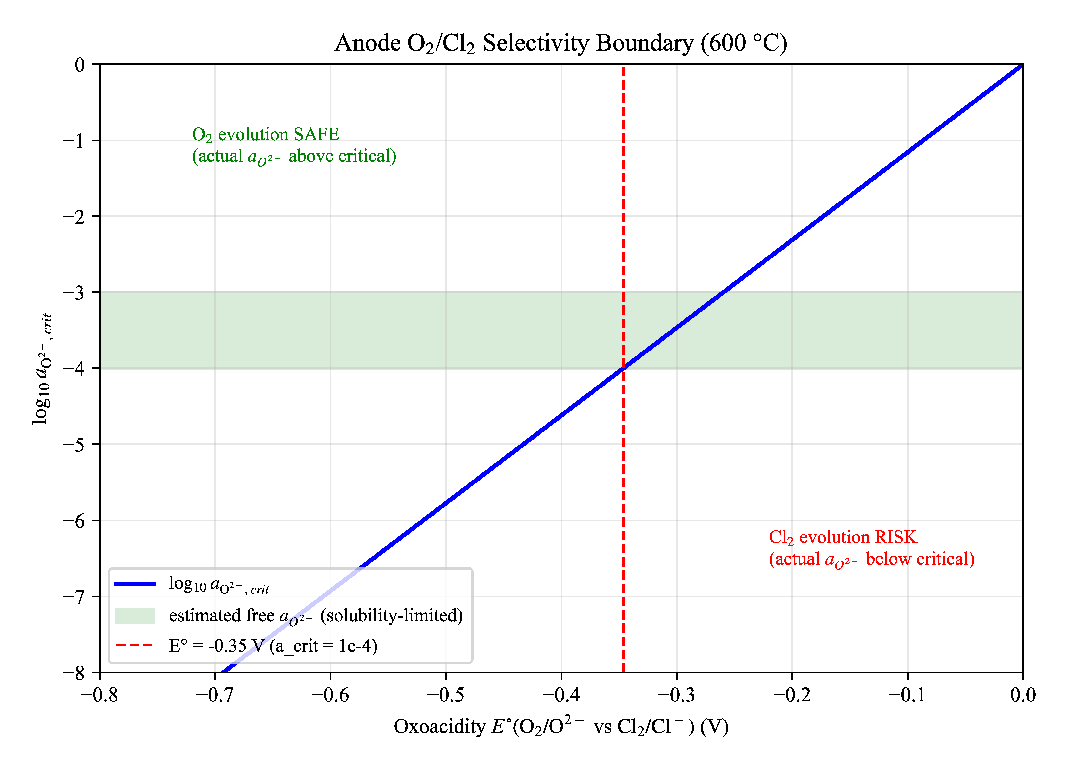
\includegraphics[width=0.85\linewidth]{figure12.eps}
\caption{Anode $\ce{O2}$/$\ce{Cl2}$ selectivity boundary at 600~$^{\circ}$C. The critical free-oxide activity $a_{\ce{O^{2-}},crit}$ (solid line) is plotted as a function of the melt oxoacidity $E^{\circ}(\ce{O2/O^{2-}}~\text{vs}~\ce{Cl2/Cl^-})$, which has not been measured for this quaternary system. The green band is the estimated operating $a_{\ce{O^{2-}}}$ from oxide solubility and $\ce{Ca^{2+}}$--$\ce{O^{2-}}$ complexation. The marked crossing ($E^{\circ} \approx -0.35$~V) is derived from the assumed $a_{\ce{O^{2-}}}$ range ($10^{-4}$--$10^{-3}$), not from any measured oxoacidity; $\ce{O2}$ evolution is thermodynamically favored only to its left.}
\label{fig:cl2}
\end{figure}

A second, coupled consequence of anode-side $\ce{Cl2}$ evolution is the chemical attack of the Ti product by dissolved chlorine. Molten-salt titanium electrochemistry is well known to suffer a ``valence cycle'' current-efficiency loss in which Ti metal reacts with $\ce{Cl2}$/$\ce{TiCl4}$ to form the soluble lower chlorides $\ce{TiCl2}$/$\ce{TiCl3}$, which are then re-oxidized at the anode, shuttling charge without net Ti production. In the present process this cycle is suppressed \emph{only} while the anode remains selective to $\ce{O2}$ (Fig.~\ref{fig:cl2}): any drift into the $\ce{Cl2}$-evolution regime not only degrades the closed-loop $\ce{O2}$ assumption but also re-introduces the dominant current-loss mechanism of chloride-based titanium electrochemistry. This further underscores that the oxoacidity---and hence the $\ce{O2}$/$\ce{Cl2}$ anode selectivity---is, together with the 600~$^{\circ}$C oxide solubility, one of the two pivotal missing measurements for the proposed process.

The thermodynamic driving force of this cycle is substantial (Table~\ref{tab:ticl}): all three titanium chlorides are strongly stable relative to the elements, and the disproportionation $\ce{Ti + TiCl4 -> 2TiCl2}$ has $\Delta G^{\circ}(298~\mathrm{K}) \approx -202$~kJ/mol, remaining exergonic ($\approx -80$~kJ/mol) at 873~K when estimated from the 298~K enthalpy/entropy of formation. Thus, whenever free $\ce{Cl2}$ or $\ce{TiCl4}$ is present, the Ti cathode product is thermodynamically unstable against dissolution as $\ce{TiCl2}$/$\ce{TiCl3}$, which then migrate to the anode and are re-oxidized---the classic current-efficiency killer of chloride-based Ti electrolysis. The proposed process suppresses this only by keeping the anode in the $\ce{O2}$ regime of Fig.~\ref{fig:cl2}.

\begin{table}[!ht]
\centering
\footnotesize
\caption{Standard Gibbs free energies of formation of titanium chlorides (Barin \cite{barin1995}, 298~K, approximate) and the $\ce{Ti + TiCl4 -> 2TiCl2}$ disproportionation.}
\label{tab:ticl}
\begin{tabular}{lc}
\toprule
Species / reaction & $\Delta G^{\circ}$ (kJ/mol) \\
\midrule
$\ce{TiCl2(s)}$ & $-464$ \\
$\ce{TiCl3(s)}$ & $-654$ \\
$\ce{TiCl4(g)}$ & $-727$ \\
$\ce{Ti + TiCl4 -> 2TiCl2}$ (298~K) & $-202$ \\
$\ce{Ti + TiCl4 -> 2TiCl2}$ (873~K, est.) & $\approx -80$ \\
\bottomrule
\end{tabular}

\par\footnotesize The 873~K value is estimated as $\Delta G(873) \approx \Delta H^{\circ}(298) - 873\,\Delta S^{\circ}(298)$ using the 298~K Barin enthalpy and entropy of formation (neglecting $C_p$ temperature dependence).
\end{table}

A final constraint is the moisture sensitivity of the $\ce{MgCl2}$-bearing salt: anhydrous $\ce{MgCl2}$ cannot be obtained by open thermal dehydration (hydrolysis above $\sim$200--300~$^{\circ}$C gives $\ce{MgOHCl}$ + HCl), so improperly dried salt opens a parasitic hydrogen-evolution channel and releases HCl that re-chlorinates the freshly deposited reductant \cite{song2024}. Industrial $\ce{MgCl2}$ electrolysis controls this by vacuum dehydration or chlorinating pretreatment under a dry atmosphere \cite{pletcher1990}; these standard measures are assumed here, and the dehydration energy of the small makeup-salt stream is not itemised in Table~\ref{tab:heatbal}. Moisture is therefore an avoidable engineering requirement rather than an intrinsic limitation, but it must be met before the assumed $\eta_I = 0.75$--0.80 can be pursued experimentally.

\section*{Uncertainties and Limitations}

This study is a conceptual design based on thermodynamic calculations and literature data. All quantitative results require future experimental validation; the key uncertainties are acknowledged below:

(1) \textbf{Activity coefficients}: The ideal solution assumption introduces uncertainty in the co-deposition window; the sensitivity analysis (see the Activity Coefficient Sensitivity Analysis section) suggests viability for $\gamma_{\ce{CaCl2}} = 0.3$--1.0, but precise values require FactSage/MQM calculation or direct measurement.

(2) \textbf{Electrode overpotentials and Mg/Ca co-deposition ratio}: The window analysis rests on equilibrium Nernst equations; activation overpotentials, concentration polarization and ohmic drop all modify the effective window, and the \emph{sign} of the kinetic correction is not established---the Downs cell deposits Na from a $\ce{CaCl2}$-majority melt, which suggests that $\ce{Ca^{2+}}$ reduction may instead be kinetically slower and therefore \emph{narrow} the window. Quantifying this requires exchange current densities and transfer coefficients that are unavailable for the quaternary melt. A larger uncertainty is the Mg/Ca ratio of the deposit: because Mg reduces $\sim$816~mV earlier than Ca, the equimolar alloy assumed in the material balance can only be approached when Mg deposition reaches its diffusion limit, and $D$ and $\delta$ are themselves uncertain by about an order of magnitude ($j_{\mathrm{lim,Mg}} = 0.07$--3.4~A/cm$^2$; Fig.~\ref{fig:current_regimes}), so the design current density must be established electrochemically.

(3) \textbf{SCM kinetics}: The model assumes pure diffusion control with constant $D$, neglecting convection and electromigration, and the nominal $D = 2.0\times10^{-9}$~m$^2$/s is an order-of-magnitude estimate from FFC literature data \cite{fray2000,yan2007}; the rate-limiting species (Mg/Ca inward versus O$^{2-}$ outward) remains unidentified. Multi-parameter sensitivity ($D$, $\varepsilon$, $\tau$) gives 1.3--63~min, so product-layer microstructure dominates the uncertainty. The model further assumes the porous Ti layer stays open and wetted by the liquid reductant; if the alloy blocks the pores or the layer coarsens at 600~$^{\circ}$C, $D_{\mathrm{eff}}$ could fall towards the solid-state value ($\sim$10$^{-12}$~m$^2$/s) and the reduction time lengthen from minutes to hours. Mg and Ca are essentially immiscible with Ti (no Mg--Ti or Ca--Ti intermetallics in the assessed binaries \cite{hallstedt2025}), so interfacial compound formation is not expected, but wetting, pore clogging and morphology evolution remain unquantified.

(4) \textbf{Liquidus calculation}: The ideal-solution model neglects intermediate compounds; the $\pm$50~$^{\circ}$C uncertainty allows an actual liquidus up to $\sim$594~$^{\circ}$C, leaving only $\sim$6~$^{\circ}$C below the 600~$^{\circ}$C design point---insufficient for the $\pm$10--20~$^{\circ}$C fluctuations typical of industrial electrolytic cells. If the liquidus lies near 594~$^{\circ}$C the operable window shrinks to $\sim$620--650~$^{\circ}$C (the ceiling being set by Mg melting and accelerated corrosion), and local freezing or short-circuiting becomes a pilot-fatal risk. A hard operating floor of $\geq$620~$^{\circ}$C---or CALPHAD/DSC confirmation of a substantially lower liquidus---should therefore be adopted as a design requirement.

(5) \textbf{Mg--Ca interaction parameter}: The regular solution approximation ($\Omega \approx L_0(T)$) neglects the non-symmetric $L_1$ term; the full Redlich--Kister expansion \cite{zhang2008mgce} should be used for accurate temperature-dependent calculations.

(6) \textbf{Oxide solubility at operating temperature}: The MgO solubility data (2.35~wt\%) was measured at 800~$^{\circ}$C \cite{morita2004}; Arrhenius extrapolation suggests solubility at 600~$^{\circ}$C may be approximately 0.5--1.2~wt\% (20--50\% of the 800~$^{\circ}$C value), increasing the required salt circulation rate by 2--4$\times$ but not invalidating the closed-loop concept. This is an order-of-magnitude estimate based on single-point extrapolation; the activation energy is not independently determined, and the range carries a factor-of-2.4 uncertainty. Under the reconstructed mechanism, however, the design instead requires $a_{\ce{MgO}} \lesssim 5\times10^{-3}$ (Eq.~\ref{eq:amgo}) and the regenerated species is predominantly CaO, so the unresolved solubility is that of CaO rather than of MgO.

(7) \textbf{Impurity separation}: Fe--Ti and Si--Ti form intermetallic compounds at 600~$^{\circ}$C, which may complicate gravity-based separation. The ``post-treatment'' item (300~kWh/ton, Table~\ref{tab:heatbal}) covers only salt washing, drying and screening and is \emph{distinct from} impurity removal: if metallurgical-grade $\ce{TiO2}$ ($\geq$90~wt\%) is used, $\sim$5--10~wt\% impurity metals (mainly Fe and Si) must be separated, and acid leaching of 100~$\mu$m Ti powder typically costs $\sim$200--500~kWh/ton-Ti ($\sim$2--4\% of the net energy). This is not included in the present figure and belongs in a future cradle-to-gate analysis.

(8) \textbf{Engineering factors}: Anode lifetime, current-efficiency degradation and impurity accumulation all require pilot-scale testing. Anode corrosion is the key challenge: at 600~$^{\circ}$C in chloride melts containing dissolved oxides, candidate inert anodes (SnO$_2$, RuO$_2$-coated Ti, dimensionally stable anodes, $\ce{NiFe2O4}$, $\ce{CeO2}$-coated Ni alloys) face attack by O$^{2-}$ and Cl$^-$ and degradation by the oxygen-evolution reaction. A consumable graphite anode is the fallback, at the cost of carbon contamination, $\ce{CO2}$/CO evolution, a $\sim$0.3~V higher cell voltage ($\approx$4.3~V) and a net consumption rising from 12{,}552 to $\sim$13{,}100~kWh/ton-Ti ($\sim$5\%), which would break the ``green $\ce{O2}$'' narrative while preserving the cathodic mechanism. Anode-material screening should therefore precede any commitment to the inert-anode energy balance.

(9) \textbf{Current efficiency assumption}: The assumed $\eta_I = 0.75$--0.80 rests on analogy with dissolved-salt electrolysis (Downs, Hall--H\'eroult, industrial $\ce{MgCl2}$ electrolysis) rather than on measurement, and the loss estimates given in the Material and Energy Balance section are rough. If $\eta_I$ is only 0.50--0.60 the energy consumption rises to 15{,}200--19{,}600~kWh/ton-Ti, within the FFC range, so the Monte Carlo median of 13{,}141~kWh/ton-Ti and $P(W_{\mathrm{net}} < 15{,}000) = 82.1\%$ largely restate the assumed prior. Current efficiency is the dominant uncertainty ($\rho = -0.85$) and its measurement is the most critical prerequisite for the energy claim.

(10) \textbf{Ca--MgO interfacial kinetics}: Ca reduces MgO thermodynamically (Eq.~\ref{eq:camgo}, $\Delta G^{\circ}(873~\mathrm{K}) = -38.2$~kJ/mol), so the steady-state partition of oxygen between Mg and Ca depends on the competition between MgO dissolution/electrolytic regeneration and its chemical reduction by the alloy at the alloy/salt interface. Neither the interfacial rate of reaction~\ref{eq:camgo} nor the MgO dissolution kinetics at 600~$^{\circ}$C is known. The 1:1 material balance of Table~\ref{tab:mbalance} assumes the electrolytic pathway dominates; the opposite limit (Ca as the sole net oxygen carrier) raises the net energy consumption from 12{,}552 to 12{,}933~kWh/ton-Ti. This kinetic competition is the most important unmeasured input for the mechanism, and the same balance governs the Mg inventory: Mg deposited at its diffusion limit must have an outlet (evaporation, entrainment, or periodic alloy withdrawal) if it is not to accumulate in the alloy pool. The criterion that discriminates the two cases experimentally is the interfacial rate of reaction~\ref{eq:camgo} relative to the MgO dissolution rate: if it proves slow, the 1:1 limit is recovered and the net energy falls to 12{,}552~kWh/ton-Ti, 3\% below the 12{,}933~kWh/ton-Ti CaO-only value.

(11) \textbf{Reactor engineering}: The crucible-as-current-collector configuration, the ceramic anode shroud and the periodic drainage of a 620~$^{\circ}$C slurry are conceptual. The long-term corrosion and salt-permeation resistance of candidate shroud ceramics in the quaternary melt are unquantified; failure of the shroud would re-open the soft-short-circuit path that the settled, electronically conductive Ti bed creates. Sealing and freeze-off of the bottom isolation valve, and the heat loss associated with periodic drainage, are not itemised in Table~\ref{tab:heatbal}. The slope of the cell floor is a design target rather than a measured parameter: the angle of repose of a Ti/MgO/CaO slurry in a chloride melt at 620~$^{\circ}$C is unknown, dry-powder values (30--45$^{\circ}$) bracket the 45$^{\circ}$ sometimes proposed, and $\geq$55$^{\circ}$ with gas-pulsed loosening at the port is adopted pending measurement.

(12) \textbf{Product separation chain}: The electrostatic separation of Ti from unreacted $\ce{TiO2}$, the liberation step that precedes it, and the magnetic/alkaline removal of reduced Fe and Si are standard unit operations but are not quantified here, and the efficiency of electrostatic separation below $\sim$10~$\mu$m is not established. The 300~kWh/ton post-treatment figure covers washing, drying and screening only and is distinct from these steps (see also Limitations~(7)).

\section*{Conclusions}

(1) The proposed quaternary $\ce{MgCl2-CaCl2-NaCl-KCl}$ molten salt process is designed to enable in-situ electrolytic co-deposition of Mg and Ca for complementary reduction of $\ce{TiO2}$. If the proposed bimetallic co-deposition can be realized experimentally, the process combines Ca as the thermodynamic deoxidation driver ($\ce{Ca + MgO -> CaO + Mg}$, $\Delta G^{\circ}(600~^{\circ}\mathrm{C}) = -38.2$~kJ/mol, Eq.~\ref{eq:camgo}) with Mg as the component that keeps the reductant liquid at 600~$^{\circ}$C, where both pure metals are solid: the equilibrium limits are 3908~ppm O for Mg acting alone versus 20.2~ppm for Ca (193$\times$), the latter becoming $\approx$77~ppm at the equimolar alloy activity---far below the 0.10--0.20~wt\% commercial target, provided the dissolved MgO activity is held below $\approx 5\times10^{-3}$ (Eq.~\ref{eq:amgo}).

(2) The $\ce{Ca^{2+}/Na+}$ co-deposition window is 120.2~mV (ideal) and remains positive (74.9--147.1~mV) for $\gamma_{\ce{CaCl2}} = 0.3$--1.0, with the critical $\gamma_{\ce{CaCl2}}$ at $\sim$0.02--0.04; the kinetic correction to this equilibrium window is not yet signed, since Downs-cell evidence suggests it may narrow rather than widen the window. A diffusion-layer analysis ($D = 1.0\times10^{-9}$~m$^2$/s, $\delta = 200~\mu$m) places Mg--Ca co-deposition between the Mg limiting current (0.56~A/cm$^2$) and the $\ce{Na+}$ onset (1.31~A/cm$^2$), with the equimolar deposit at $j \approx 1.1$~A/cm$^2$; the 0.9~V ohmic budget then constrains the interelectrode gap to $\lesssim$1.1~cm at $\kappa = 1.4$~S/cm, dictating a close-spaced or diaphragm-integrated cell.

(3) The Mg--Ca liquid alloy, described by the regular solution approximation from Zhang et al. (2008) CALPHAD assessment ($\Omega \approx L_0 = -18.64$~kJ/mol at 873~K, $\Delta G_{\mathrm{mix}} = -9.69$~kJ/mol at equimolar), is thermodynamically stable, favoring homogeneous co-deposition.

(4) SCM kinetics estimate 100~$\mu$m-diameter particle complete reduction in 6.3~min ($R = 50~\mu$m, $D = 2.0\times10^{-9}$~m$^2$/s), with sensitivity analysis ($D = 1$--$3\times10^{-9}$~m$^2$/s) yielding 4.2--12.7~min. E--$p\ce{O^{2-}}$ diagrams indicate preferential Fe/Si reduction, suggesting potential compatibility with metallurgical-grade $\ce{TiO2}$ feedstock.

(5) Full-process energy balance gives 12{,}552~kWh/ton-Ti net equivalent consumption at the nominal design point ($\eta_I = 0.75$, $V_{\mathrm{cell}} = 4.1$~V; \emph{theoretical prediction, conditional on achieving $\eta_I > 0.70$}; heat-integration credit capped at the 329~kWh/ton-Ti external thermal demand, with the reaction exotherm rejected as cell waste heat; excluding impurity separation, which may add $\sim$2--4\%). The process energy efficiency (electrolysis step minimum / net equivalent consumption) is 48.7\%, and the second-law efficiency is $\sim$36.3\% (net reaction reversible work 4{,}550~kWh/ton-Ti / net equivalent consumption). The electrolysis energy fraction is 97.2\%. If Ca acts as the sole net oxygen carrier (CaO regeneration, Eq.~\ref{eq:camgo}), the decomposition voltage rises from 2.73 to 2.83~V and the net equivalent consumption to 12{,}933~kWh/ton-Ti ($+$3\%); this CaO-only limit is the mechanistically favoured case, because reaction~\ref{eq:camgo} generates no solid product layer to retard it, while the 1:1 balance is retained as the conservative design basis. If $\eta_I = 0.50$--0.60, net equivalent consumption rises to $\sim$15{,}200--19{,}600~kWh/ton-Ti, within the FFC range.

(6) A Monte Carlo analysis ($N = 10^5$, $\eta_I \sim \mathrm{Tri}(0.50, 0.75, 0.88)$) gives a median $W_{\mathrm{net}}$ of 13{,}141~kWh/ton-Ti under the conservative 1:1 basis (13{,}536~kWh/ton-Ti under the CaO-only basis) and a probability $P(W_{\mathrm{net}} < 15{,}000)$ of 82.1\% (76.6\% under the CaO-only basis) relative to the FFC lower bound; that probability largely restates the assumed $\eta_I$ prior rather than providing an independent feasibility estimate. Current efficiency is the dominant uncertainty ($\rho = -0.85$), so its experimental validation is the most critical prerequisite. The Hall--H\'eroult analogy ($\eta_I = 90$--95\%) \cite{kvande2014} is a reference point, not a validation, since the two processes differ in decomposition voltage, cathode product state, oxide solubility and anode conditions.

(7) Two critical assumptions require experimental validation before pilot-scale implementation: \textbf{(a)} the liquidus calculation (ideal solution model, $\pm$50~$^{\circ}$C uncertainty) must be verified by CALPHAD assessment or DSC measurement---the current 580~$^{\circ}$C operating lower bound should be regarded as a target design value, not a validated operating limit; \textbf{(b)} the closed-loop salt circulation depends on adequate oxide solubility at 600~$^{\circ}$C, currently estimated by Arrhenius extrapolation from 800~$^{\circ}$C data without confidence intervals---if the actual solubility falls below 0.5~wt\%, the salt circulation rate would need to increase by more than 4$\times$, potentially invalidating the closed-loop design. Under the reconstructed mechanism, however, the species that must be dissolved and regenerated is predominantly CaO (Eq.~\ref{eq:camgo}), whose solubility in $\ce{CaCl2}$-rich melts exceeds that of $\ce{MgO}$, while a \emph{low} MgO solubility is itself a design requirement ($a_{\ce{MgO}} \lesssim 5\times10^{-3}$; Eq.~\ref{eq:amgo}); the pivotal missing measurements are therefore the CaO solubility and the interfacial kinetics of Eq.~\ref{eq:camgo}.

(8) All quantitative results are based on ideal solution assumptions and literature parameters; activity coefficient corrections, CALPHAD database calculations, and pilot-scale studies are needed for validation. This work provides a theoretical framework for subsequent research.

(9) As go/no-go decision criteria for subsequent pilot funding, the following bounds are proposed: (i) if the measured current efficiency falls below $\eta_I = 0.60$ at $V_{\mathrm{cell}} = 4.0$~V, the net equivalent consumption rises to $\sim$15{,}200~kWh/ton-Ti, eliminating the net energy advantage over the FFC route (15{,}000--20{,}000~kWh/ton-Ti); and (ii) if the 600~$^{\circ}$C oxide solubility is confirmed below 0.5~wt\%, the salt inventory exceeds $\sim$400~t per ton Ti and the closed loop becomes impracticable. In either case, the closed-loop design should be reconsidered (e.g., a simpler open-loop Mg-reduction variant) rather than progressed to pilot scale.

(10) The preferred cell is a semi-continuous reactor in which a settled $\ce{TiO2}$ bed on a sloped floor forms the cathode, the reductant is electrodeposited within the bed and retained there by capillarity, an anode suspended in the clear melt above is enclosed in a ceramic shroud, and the Ti/MgO/CaO slurry is drained periodically through a bottom isolation valve while fresh $\ce{TiO2}$ is fed to the bed surface. The interelectrode gap is set by the ohmic budget at $\lesssim$1.1~cm, so short-circuit protection must be geometric rather than dimensional. Screening alone cannot separate the Ti product from unreacted $\ce{TiO2}$ of the same particle size; dry electrostatic separation, exploiting the conductivity contrast, is the proposed primary step, with the oxide fraction returned to the cell.

\noindent\textbf{Declarations}

\noindent\textbf{Data Availability}: All thermodynamic data are from the cited literature. The Python scripts used for calculations and figure generation are publicly available at \url{https://github.com/huyamingc/ti-in-situ-electrolysis}. A preprint version of this work has been deposited on Zenodo (DOI: \href{https://doi.org/10.5281/zenodo.21973469}{10.5281/zenodo.21973469}).

\noindent\textbf{Conflict of Interest}: The author declares no conflict of interest.

\noindent\textbf{Author Contributions}: Yaming Hu: Conceptualization, Methodology, Formal analysis, Investigation, Writing---original draft, Writing---review \& editing, Visualization.

\noindent\textbf{Funding}: This research did not receive any specific grant from funding agencies in the public, commercial, or not-for-profit sectors.

\begin{thebibliography}{99}

\bibitem{kroll1937} W. J. Kroll, Z. Anorg. Allg. Chem., 234, 42 (1937).

\bibitem{ji2026} H. Ji, S. Guo, L. Gao, L. Yang, H. Yan, and H. Zeng, Int. J. Miner. Metall. Mater., 33, 15 (2026).

\bibitem{fray2000} G. Z. Chen, D. J. Fray, and T. W. Farthing, Nature, 407, 361 (2000).

\bibitem{jiao2023} H. Jiao, M. Liu, Z. Wang, M. Lin, Z. Qu, J. Song, and S. Jiao, ACS Sustainable Chem. Eng., 11, 5764 (2023).

\bibitem{ono2002} K. Ono and R. O. Suzuki, JOM, 54, 59 (2002).

\bibitem{pal2001} U. B. Pal, D. E. Woolley, and G. B. Kenney, JOM, 53, 32 (2001).

\bibitem{okabe1997} T. H. Okabe and Y. Waseda, JOM, 49, 28 (1997).

\bibitem{zhang2024} J. Zhang, H. Yan, Z. Liu, S. Guo, Y. Yang, G. Yang, R. Xia, M. Hu, and L. Li, J. Electrochem. Soc., 171, 082502 (2024).

\bibitem{taninouchi2016} Y. Taninouchi, Y. Hamanaka, and T. H. Okabe, Metall. Mater. Trans. B, 47, 3394 (2016).

\bibitem{lee2025} K. S. Lim, H. Nersisyan, S. K. Han, K.-T. Park, H. Suh, and J. H. Lee, Next Mater., 8, 100803 (2025).

\bibitem{pang2024} J. Pang, L.-X. Kong, L.-G. Zhu, B.-Q. Xu, J.-J. Xu, C.-L. Bai, and B. Yang, Trans. Nonferrous Met. Soc. China, 34, 681 (2024).

\bibitem{xu2025} L. Zhu, Z. Zhang, L. Kong, B. Xu, and B. Yang, Electrochim. Acta, 533, 146478 (2025).

\bibitem{barin1995} I. Barin, Thermochemical Data of Pure Substances, 3rd ed., VCH, Weinheim (1995).

\bibitem{waldner1999} P. Waldner and G. Eriksson, Calphad, 23, 189 (1999).

\bibitem{zhang2008mgce} H. Zhang, Y. Wang, S. L. Shang, L.-Q. Chen, and Z.-K. Liu, J. Alloys Compd., 463, 294 (2008).

\bibitem{sato1999} Y. Sato, Y. Kuroda, T. Nagatsu, M. Hoshi, J.-I. Kim, and T. Yamamura, in Molten Salts XII, P. C. Trulove, H. C. DeLong, G. R. Stafford, and S. Deki, Editors, PV 99-41, p. 313, The Electrochemical Society Proceedings Series, Pennington, NJ (1999).

\bibitem{kubaschewski1979} O. Kubaschewski and C. B. Alcock, Metallurgical Thermochemistry, 5th ed., Pergamon Press, Oxford (1979).

\bibitem{chartrand2000} P. Chartrand and A. D. Pelton, Can. Metall. Q., 39, 405 (2000).

\bibitem{pletcher1990} D. Pletcher and F. C. Walsh, Industrial Electrochemistry, 2nd ed., Chapman and Hall, London (1990).

\bibitem{kleppa1966} O. J. Kleppa and F. G. McCarty, J. Phys. Chem., 70, 1249 (1966).

\bibitem{pelton2000mqm} A. D. Pelton, S. A. Degterov, G. Eriksson, C. Robelin, and Y. Dessureault, Metall. Mater. Trans. B, 31, 651 (2000).

\bibitem{nayeb1987} A. A. Nayeb-Hashemi and J. B. Clark, Bull. Alloy Phase Diagrams, 8, 58 (1987).

\bibitem{hallstedt2025} B. Hallstedt, Calphad, 89, 102833 (2025).
\bibitem{tang2015} H. Tang, Y. Ren, S. Wang, H. Deng, D. Cai, L. Shao, Y. Zhao, R. Gao, Y. Yan, and M. Zhang, J. Electrochem. Soc., 162, D520 (2015).
\bibitem{yan2007} X. Y. Yan and D. J. Fray, Miner. Process. Extr. Metall., 116, 17 (2007).

\bibitem{littlewood1962} R. Littlewood, J. Electrochem. Soc., 109, 525 (1962).

\bibitem{levenspiel1999} O. Levenspiel, Chemical Reaction Engineering, 3rd ed., Wiley, New York (1999).

\bibitem{kvande2014} H. Kvande and P. A. Drabl{\o}s, J. Occup. Environ. Med., 56, S23 (2014).

\bibitem{morita2004} M. Ito and K. Morita, Mater. Trans., 45, 2712 (2004).

\bibitem{song2024} Z. Song, J. Zhao, Z. He, and G. Lu, J. Electrochem. Soc., 171, 062501 (2024).

\end{thebibliography}

\end{document}
